%-------------------------------------------------------------------------------
% Edge detectors review
% by Haldo Spontón & Juan Cardelino
% IPOL 2012
%-------------------------------------------------------------------------------
\documentclass{ipol}
\ipolSetYear{2012}
\ipolSetDOI{10.XXXX/ipol.2012.sc-red}

\usepackage{hyperref,verbatim,graphicx,amsmath,amssymb,amssymb,dsfont}
\usepackage[ruled,linesnumbered]{algorithm2e}
\usepackage{sidecap,subfig,array}
\usepackage[table]{xcolor}
\usepackage{multicol}
\usepackage{listings}
\usepackage{color}
\newtheorem{theorem}{Theorem}
\numberwithin{equation}{section}
\numberwithin{table}{section}
\numberwithin{figure}{section}
\begin{document}
\bibliographystyle{ieeetr}
\lstset{
	backgroundcolor=\color[rgb]{0.9,0.9,0.9},
    tabsize=4,
    inputencoding=utf8x,
         extendedchars=\true,
         language=C++,
         basicstyle=\scriptsize,
                 showtabs=false,
        showspaces=false,
        showstringspaces=false,
        identifierstyle=\ttfamily,
        keywordstyle=\color[rgb]{0,0,1},
        commentstyle=\color[rgb]{0.133,0.545,0.133},
        stringstyle=\color[rgb]{0.627,0.126,0.941},
}

%-------------------------------------------------------------------------------
\title{Review of Edge Detectors}
\author{Haldo Spont\'on,\\
        Juan Cardelino}
\date{}
\ipolMaketitle

%-------------------------------------------------------------------------------
\begin{ipolAbstract}
In this paper we study some of the classic alternatives for edge detection in digital images. The main idea 
behind the edge detection is to find where there are abrupt changes in the intensity of an image. 
As a first approach, the first derivative is used to find the changes of intensity in several algorithms 
such as Sobel, Prewitt and Roberts \cite{Gonzalez2007Digital}. The second derivative is also used, for example in algorithms 
like Marr-Hildreth \cite{AIM-518} and Haralick \cite{bb20239}.\\
We compare the results obtained from a qualitative point of view (perceptual) and from a quantitative 
point of view (number of operations, execution time), considering different forms to convolve an 
image with a kernel (step required in some of the algorithms).\\


%The Marr-Hildreth algorithm is a method of detecting edges in digital 
%images. It's based on convolving the image with the Laplacian of the 
%Gaussian function. Then, zero crossings are detected in the filtered 
%result to obtain the edges points.
\end{ipolAbstract}

%-------------------------------------------------------------------------------
\begin{ipolCode}
The C implementation of the algorithms implemented in this work (beta version) can be
downloaded from \href{http://iie.fing.edu.uy/~haldos/downloads/edge_detectors_v0.1.tar.gz}{here}.
%\begin{itemize}
%	\item Roberts, Prewitt and Sobel operators: \href{http://iie.fing.edu.uy/~haldos/ipol/fded.tar.gz}{here}.
%	\item Marr-Hildreth algorithm: \href{http://iie.fing.edu.uy/~haldos/ipol/marr-hildreth.tar.gz}{here}.
%	\item Haralick algorithm: \href{http://iie.fing.edu.uy/~haldos/ipol/haralick.tar.gz}{here}.
%\end{itemize}
% TODO referencia a github
\end{ipolCode}

%-------------------------------------------------------------------------------
%\begin{ipolSupp}
%\end{ipolSupp}

%-------------------------------------------------------------------------------
\section{Introduction}
\label{sec:intro}

Edge detection is one of the first approaches published in the literature for 
segmenting images. The basic idea is to detect abrupt changes in intensity. 
Detecting those changes in intensity for the purpose of finding edges in images 
can be accomplished using first or second order derivatives. \\

In the 70's, edge detection methods were based on using small operators 
(such as Sobel masks), attempting to compute an approximation of the
first derivative of the image. In section ~\ref{sec:first} we study the 
performance of such algorithms, as an introduction to a more sophisticated 
analysis into the edge finding process.\\

In 1980 Marr and Hildreth argued that intensity changes are not independent 
of image scale, so the edge detection requires the use of different size 
operators. They also argued that a sudden intensity change will be seen 
as a peak (or trough) in the first derivative or, equivalently, as a zero 
crossing in the second derivative. The bulk of this work focuses on the 
study of this algorithm, presented in Section ~\ref{sec:second}. In this section 
we also present the Haralick algorithm, which is also based on the second derivative.
This algorithm has the particularity of proposing a model to locally approximate 
the image around a point. Then, with this model, second derivative can be calculated 
analytically (rather approximate) and finding edges is done by imposing a 
condition over the model parameters. \\

Results and conclusions are shown in sections \ref{sec:results} and 
\ref{sec:conclusions} respectively. In section ~\ref{sec:examples} we present some examples to compare the 
performance of the algorithms studied in this work. We also present a 
video created using the implemented algorithms, applied frame by frame.\\

%-------------------------------------------------------------------------------
\section{Algorithms based on first derivative}
\label{sec:first}

The usual tool to find the amplitude and direction of changes in 
intensity of an image $f$ is the gradient operator (denoted as $\nabla$), defined 
as the vector:
\begin{equation}
	\nabla f = 
				\begin{bmatrix} 
					g_x \\ g_y
				\end{bmatrix}
	=				
				\begin{bmatrix} 
					\cfrac{\partial f}{\partial x} \\ \cfrac{\partial f}{\partial y} \\
				\end{bmatrix}
\end{equation}

The magnitude ($M$) and direction ($\alpha$) of the gradient vector $\nabla f$ at location $(x,y)$
are calculated as:
\begin{equation}
	\begin{cases}
		M(x,y) = \sqrt{g_x^2 + g_y^2} \\
		\alpha(x,y) = \tan^{-1} \begin{bmatrix} g_x \\ g_y \end{bmatrix} \\
	\end{cases}
\end{equation}

The direction of an edge at an arbitrary location $(x,y)$ of the image is 
orthogonal to the direction $\alpha(x,y)$ of the gradient vector.\\

We need to compute partial derivatives $\partial f/\partial x$ and $\partial f/\partial y$ 
at every pixel in the image. Since we are dealing with digital images, numerical approximations 
of the partial derivatives over a neighborhood about a point are required. In the following we will study 
the methods of Roberts, Prewitt and Sobel, whose main difference is how they perform this calculation.\\

\subsection{The \textit{Roberts} operators}

The most usual approach of the first derivative is to take the Taylor expansion of first order with
a small $h$. Approximating the first derivative:
\begin{equation}
	f'(x) \simeq \frac{f(x+h) - f(x)}{h}\\
\end{equation}
The image has discrete points of coordinates $(i,j)$, so taking $x=i*h$ and $y=j*h$, we approximate the 
first derivative of the image based on the intensity values ​​at points of the image as:
\begin{equation}
\label{eq:roberts1}
	g_x = \frac{\partial f(x,y)}{\partial x} = f(i+1,j) - f(i,j)
\end{equation}
and
\begin{equation}
\label{eq:roberts2}
	g_y = \frac{\partial f(x,y)}{\partial y} = f(i,j+1) - f(i,j)\\
\end{equation}

Equations \ref{eq:roberts1} and \ref{eq:roberts2} can be implemented for all values of $x$ and $y$
by filtering the image $f(x,y)$ with the 1-D masks in figure \ref{fig:1dmasks}. But when we want 
to find diagonal edges, we need 2-D masks. The \textit{Roberts operators} are one of the earliest 
attempts to use 2-D masks for this purpose. These operators are based on implementing the diagonal 
diferences implemented by filtering an image with the masks in figure \ref{fig:roberts}.\\

\begin{SCfigure}[3][!h]
	\centering
	\includegraphics[width=0.14\textwidth]{1dmasks.pdf}
	\caption{One-dimensional masks used to implement equations \ref{eq:roberts1} and \ref{eq:roberts2}.}
	\label{fig:1dmasks}
\end{SCfigure}

\begin{SCfigure}[3][!h]
	\centering
	\includegraphics[width=0.15\textwidth]{roberts.pdf}
	\caption{\textit{Roberts cross-gradient} 2-D masks.}
	\label{fig:roberts}
\end{SCfigure}

\subsection{The \textit{Prewitt} operators}

Masks of size $2\times2$ are conceptually simple, but not being symmetrical to a central point implies 
that they are not as useful for detecting edges as symmetrical ones. The smaller mask with these characteristics is 
$3\times3$. These masks provide more information to find the direction of the edges, because they take 
into account information on opposite sides of the central point.\\

The simplest digital approximation to the partial derivatives using masks of size $3\times3$ are given 
by taking the difference between the third and first rows (or columns) of the $3\times3$ region. The
difference between the third and first rows approximates the derivative in the x-direction, and 
the difference between the third and first columns approximates the derivative in the y-direction.
These approximations can be implemented by filtering the image with the two masks in figure \ref{fig:prewitt}.
These masks are called \textit{Prewitt operators}.\\

\begin{SCfigure}[2][!h]
	\centering
	\includegraphics[width=0.25\textwidth]{prewitt.pdf}
	\caption{\textit{Prewitt} 2-D masks of size $3\times3$.}
	\label{fig:prewitt}
\end{SCfigure}

\subsection{The \textit{Sobel} operators}

A slight variation of the Prewitt operators use more weight on the central coefficients of the 
difference. It can be shown that using a $2$ in the center location provides image smoothing. This
variation is implemented using masks in figure \ref{fig:sobel}. These operators are called 
\textit{Sobel operators}.\\

\begin{SCfigure}[2][!h]
	\centering
	\includegraphics[width=0.25\textwidth]{sobel.pdf}
	\caption{\textit{Sobel} 2-D masks of size $3\times3$.}
	\label{fig:sobel}
\end{SCfigure}

The Prewitt masks are simpler to implement than the Sobel masks, but the computational difference
between them is not an issue. It is preferable to use Sobel operators, because they have better
noise-suppression characteristics (smoothing). Noise suppression is an important issue when dealing
with derivatives.\\

%-------------------------------------------------------------------------------
\section{Algorithms based on second derivative}
\label{sec:second}

The edge detection methods discussed in the previous section are simply based on filtering the 
image with different masks, without taking into account the characteristics of the edges or 
noise in the image.\\

The two algorithms that we will see in this section (Marr-Hildreth [1980] and Haralick [1987]) 
are based on the second derivative of the image, and both take steps to reduce noise before 
detecting edges in the image.\\

\subsection{The \textit{Marr} and \textit{Hildreth} algorithm}

The Marr-Hildreth algorithm is a method of detecting edges in digital 
images. It's based on find zero crossing points of the second derivative
of the image. This can be done in several ways. In this work we implemented 
two different ways; convolving the image with a Gaussian kernel and then 
approximating the second derivative (Laplacian) with a 3x3 kernel, or 
convolving the image with a kernel calculated as the Laplacian of a 
Gaussian function. There are more ways to do so, for example, using 
recursive Gaussian filters.\\ % poner referencia!

The algorithm is divided in three steps, each one described later:
\begin{enumerate}
	\item Grayscale conversion of the input image (see section \ref{sec:appendix1}).
	\item Convolution of the image with:
	\begin{itemize}
		\item a Laplacian of Gaussian (LoG) kernel. (or)
		\item a Gaussian kernel and then a Laplacian operator.
	\end{itemize}
	\item Search of zero crossing points in the filtered image.\\
\end{enumerate}

Some auxiliary functions were implemented for computing the operations
needed in the algorithm, such as Gaussian kernel and Laplacian of a Gaussian 
kernel generation, and 2-D convolution of an image with a given kernel, 
with zero padding.\\



%-------------------------------------------------------------------------------
\subsubsection{Gaussian and LoG kernels}

The Marr-Hildreth algorithm consists of convolving the LoG filter with an input image, $f(x,y)$.
\begin{equation}\label{eq:log}
  g(x,y) = [\nabla^2G(x,y)]\star f(x,y)
\end{equation}
and then finding the zero crossings of $g(x,y)$ to determine the location of edges in $f(x,y)$. 
Because these are linear processes, equation \ref{eq:log} can be written also as
\begin{equation}
  g(x,y) = \nabla^2[G(x,y)\star f(x,y)]
\end{equation}
indicating that we can smooth the image first with a Gaussian filter and then compute the Laplacian of the result.\\

Then we need to generate both Gaussian kernel and LoG kernel (see section \ref{sec:appendix2}).\\

The Marr-Hildreth edge-detection algorithm may be summarized as follows:
\begin{enumerate}
	\item Filter the input image with a $n \times n$ Gaussian lowpass filter obtained by sampling equation \ref{eq:gaussian_function}.
	\item Compute the Laplacian of the image resulting from step 1, using, for example, the $3\times3$ mask:
			$\begin{bmatrix}
			1 &  1 & 1 \\
			1 & -8 & 1 \\
			1 &  1 & 1 \\
			\end{bmatrix}$\footnote{Steps 1 and 2 can be made into one, using a $n\times n$ LoG lowpass filter obtained by sampling equation \ref{eq:log_function}.}
	\item Find the zero crossings of the image from step 2.
\end{enumerate}

%-------------------------------------------------------------------------------
\subsubsection{Zero crossing}

A zero crossing at pixel $p$ implies that the signs of at least two opposite neighboring pixels are 
different. There are four cases to test: left/right, up/down, and the two diagonals. In this case 
we work with a threshold, so that not only the signs of the opposite pixels must differ, also their 
difference in absolute value must be greater than a certain threshold.\\

Zero crossing detection is the key feature of the Marr-Hildreth edge detection method. The technique 
presented in the previous paragraph is attractive for its simplicity of implementation and its low 
computational cost. In general it is a technique that yields good results, but if more precision in 
finding the zero crossings is needed, methods for finding zero crossings with subpixel accuracy 
should be used.\\

%-------------------------------------------------------------------------------
\subsection{The \textit{Haralick} algorithm}

The idea behind the Haralick edge detector is identical to that of the previous method; find zeros in 
the second derivative of the image. In this method, we smooth the input image through local bi-cubic
polynomial fitting. Then, calculating the second derivative analytically, we can find an expression 
equivalent to cancel the second derivative of the polynomial as a function of the parameters of it.\footnote{This implementation is slightly 
different to the traditional implementation of the Haralick algorithm. We do not use the condition concerning the third derivative.}\\

\subsubsection{Bi-cubic polynomial fitting}
\label{sec:bicubic}

We adjust the surrounding neighborhood of a point $(x,y)$ in the image $f$ using the following bi-cubic polynomial:
\begin{equation}
	\label{eq:bicubic}
	f(x,y) = k_1 + k_2x + k_3y + k_4x^2 + k_5xy + k_6y^2 + k_7x^3 + k_8x^2y + k_9xy^2 + k_{10}y^3\\
\end{equation}

To solve this problem, we need to take more neighbors than coefficients to be adjusted. The smallest 
neighborhood of odd dimensions has size $5\times5$. Now it is possible to convolve the input image
with some precomputed masks, instead of finding the least square solution to find the coefficients 
$k_1\dots k_{10}$ at each point $(x,y)$.\\

Consider 25 points in a small neighborhood of a point $(x,y)$ in the image. We use a least square
formulation to obtain the coefficients (25 points give equal number of equations):

\begin{equation*}
	\begin{array}{l}
		f_1 = f(x_1,y_1) = k_1 + k_2x_1 + k_3y_1 + k_4x_1^2 + k_5x_1y_1 + k_6y_1^2 + k_7x_1^3 + k_8x_1^2y_1 + k_9x_1y_1^2 + k_{10}y_1^3\\
		f_2 = f(x_2,y_2) = k_1 + k_2x_2 + k_3y_2 + k_4x_2^2 + k_5x_2y_2 + k_6y_2^2 + k_7x_2^3 + k_8x_2^2y_2 + k_9x_2y_2^2 + k_{10}y_2^3\\
		\vdots \\
		f_{25} = f(x_{25},y_{25}) = k_1 + k_2x_{25} + k_3y_{25} + k_4x_{25}^2 + k_5x_{25}y_{25} + k_6y_{25}^2 + k_7x_{25}^3 + k_8x_{25}^2y_{25} + k_9x_{25}y_{25}^2 + k_{10}y_{25}^3\\
	\end{array}
\end{equation*}

Using matrix notation:

\begin{equation*}
	\begin{bmatrix} 
		f_1		\\ 
		f_2		\\ 
		\vdots	\\
		f_{25}
	\end{bmatrix} 
	= 
	\begin{bmatrix} 
		1 		& x_1 		& y_1 		& x_1^2 	& x_1y_1 		& y_1^2 	& \hdots 	& y_1^3 	\\
		1 		& x_2 		& y_2 		& x_2^2 	& x_2y_2 		& y_2^2 	& \hdots 	& y_2^3 	\\
		\vdots	& \vdots	& \vdots	& \vdots	& \vdots		& \vdots	& \ddots	& \vdots	\\
		1 		& x_{25}	& y_{25}	& x_{25}^2 	& x_{25}y_{25} 	& y_{25}^2 	& \hdots 	& y_{25}^3
	\end{bmatrix}
	\times
	\begin{bmatrix}
		k_1		\\
		k_2		\\
		\vdots	\\
		k_{10}
	\end{bmatrix}
	\Rightarrow \mathbf{f} = \mathbf{A}\mathbf{k}\\
\end{equation*}

Then:

\begin{equation*}
	(\mathbf{A}^T\mathbf{A})^{-1}\mathbf{A}^T\mathbf{f} = \mathbf{k} \ \ \Rightarrow \ \ \mathbf{k} = \mathbf{B}\mathbf{f}\\
\end{equation*}

$\mathbf{B}$ is a $10\times25$ matrix: 

\begin{equation*}
	\begin{bmatrix}
		b_{1,1}		& b_{1,2}	& \hdots	& b_{1,25}	\\
		b_{2,1}		& b_{2,2}	& \hdots	& b_{2,25}	\\
		\vdots		& \vdots	& \ddots	& \vdots	\\
		b_{10,1}	& b_{10,2}	& \hdots	& b_{10,25}
	\end{bmatrix}
	\times
	\begin{bmatrix}
		f_1		\\
		f_2		\\
		\vdots	\\
		f_{25}
	\end{bmatrix}
	=
	\begin{bmatrix}
		k_1		\\
		k_2		\\
		\vdots	\\
		k_{10}
	\end{bmatrix}\\
\end{equation*}

For each coefficient ($i$ from $1$ to $10$):

\begin{equation}
	\label{eq:coefficients}
	k_i = b_{i,1}f_1 + b_{i,2}f_2 + b_{i,3}f_3 + \hdots + b_{i,25}f_{25} \ \ \Rightarrow \ \ \mathbf{k_i} = \mathbf{f}\star\mathbf{b_i}\\
\end{equation}

where:

\begin{equation}
	\label{eq:b_i}
	\mathbf{b_i} = \begin{bmatrix}	b_{i,1}		& b_{i,2}	& \hdots	& b_{i,5}	\\
									b_{i,6}		& b_{i,7}	& \hdots	& b_{i,10}	\\
									\vdots		& \vdots	& \ddots	& \vdots	\\
									b_{i,21}	& b_{i,22}	& \hdots	& b_{i,25}	\\
					\end{bmatrix}\\
\end{equation}

Using equation \ref{eq:coefficients} and the masks given in table \ref{table:b_i}, we can compute 
the coefficients $k_1 \hdots k_{10}$ for all the points in the image. The elements of the mask $\mathbf{b_i}$ 
are the elements of the i-th row of $\mathbf{B} = (\mathbf{A}^T\mathbf{A})^{-1}\mathbf{A}^T$.\\

\newcolumntype{C}{>{\centering\arraybackslash}m{1cm}<{}}
\begin{table}
\centering
\subfloat[$\mathbf{b_1}$.] {
\begin{tabular}{|*{5}{C|}}
\hline
425 & 275 & 225 & 275 & 425 \\
\hline
275 & 125 &  75 & 125 & 275 \\ 
\hline
225 &  75 &  25 &  75 & 225 \\
\hline
275 & 125 &  75 & 125 & 275 \\
\hline
425 & 275 & 225 & 275 & 425 \\
\hline
\end{tabular}}
\qquad\qquad
\subfloat[$\mathbf{b_2}$.] {
\begin{tabular}{|*{5}{C|}}
\hline
-2260 & -620 & 0 & 620 & 2260 \\ 
\hline
-1660 & -320 & 0 & 320 & 1660 \\ 
\hline
-1460 & -220 & 0 & 220 & 1460 \\
\hline
-1660 & -320 & 0 & 320 & 1660 \\ 
\hline
-2260 & -620 & 0 & 620 & 2260 \\
\hline
\end{tabular}} \\
\subfloat[$\mathbf{b_3}$.] {
\begin{tabular}{|*{5}{C|}}
\hline
2260  &  1660 &  1460 &  1660 &  2260 \\ 
\hline
620   &   320 &   220 &   320 &   620 \\ 
\hline
0     &     0 &     0 &     0 &     0 \\
\hline
-620  &  -320 &  -220 &  -320 &  -620 \\ 
\hline
-2260 & -1660 & -1460 & -1660 & -2260 \\
\hline
\end{tabular}}
\qquad\qquad
\subfloat[$\mathbf{b_4}$.] {
\begin{tabular}{|*{5}{C|}}
\hline
1130 & 620 & 450 & 620 & 1130 \\ 
\hline
830  & 320 & 150 & 320 &  830 \\ 
\hline
730  & 220 &  50 & 220 &  730 \\
\hline
830  & 320 & 150 & 320 &  830 \\ 
\hline
1130 & 620 & 450 & 620 & 1130 \\
\hline
\end{tabular}} \\
\subfloat[$\mathbf{b_5}$.] {
\begin{tabular}{|*{5}{C|}}
\hline
-400 & -200 & 0 &  200 &  400 \\ 
\hline
-200 & -100 & 0 &  100 &  200 \\ 
\hline
0    &    0 & 0 &    0 &    0 \\
\hline
200  &  100 & 0 & -100 & -200 \\ 
\hline
400  &  200 & 0 & -200 & -400 \\
\hline
\end{tabular}}
\qquad\qquad
\subfloat[$\mathbf{b_6}$.] {
\begin{tabular}{|*{5}{C|}}
\hline
1130 & 830 & 730 & 830 & 1130 \\ 
\hline
620  & 320 & 220 & 320 &  620 \\ 
\hline
450  & 150 &  50 & 150 &  450 \\
\hline
620  & 320 & 220 & 320 &  620 \\ 
\hline
1130 & 830 & 730 & 830 & 1130 \\
\hline
\end{tabular}} \\
\subfloat[$\mathbf{b_7}$.] {
\begin{tabular}{|*{5}{C|}}
\hline
-8260 & -2180 & 0 & 2180 & 8260 \\ 
\hline
-6220 & -1160 & 0 & 1160 & 6220 \\ 
\hline
-5540 &  -820 & 0 &  820 & 5540 \\
\hline
-6220 & -1160 & 0 & 1160 & 6220 \\ 
\hline
-8260 & -2180 & 0 & 2180 & 8260 \\
\hline
\end{tabular}}
\qquad\qquad
\subfloat[$\mathbf{b_8}$.] {
\begin{tabular}{|*{5}{C|}}
\hline
5640  &  3600 &  2920 &  3600 &  5640 \\ 
\hline
1800  &   780 &   440 &   780 &  1800 \\ 
\hline
0     &     0 &     0 &     0 &     0 \\
\hline
-1800 &  -780 &  -440 &  -780 & -1800 \\ 
\hline
-5640 & -3600 & -2920 & -3600 & -5640 \\
\hline
\end{tabular}} \\
\subfloat[$\mathbf{b_9}$.] {
\begin{tabular}{|*{5}{C|}}
\hline
-5640 & -1800 & 0 & 1800 & 5640 \\ 
\hline
-3600 &  -780 & 0 &  780 & 3600 \\ 
\hline
-2920 &  -440 & 0 &  440 & 2920 \\
\hline
-3600 &  -780 & 0 &  780 & 3600 \\ 
\hline
-5640 & -1800 & 0 & 1800 & 5640 \\
\hline
\end{tabular}}
\qquad\qquad
\subfloat[$\mathbf{b_{10}}$.] {
\begin{tabular}{|*{5}{C|}}
\hline
8260  &  6220 &  5540 &  6220 &  8260 \\ 
\hline
2180  &  1160 &   820 &  1160 &  2180 \\ 
\hline
0     &     0 &     0 &     0 &     0 \\
\hline
-2180 & -1160 &  -820 & -1160 & -2180 \\ 
\hline
-8260 & -6220 & -5540 & -6220 & -8260 \\
\hline
\end{tabular}} \\
\caption{Masks to compute the coefficients of the bicubic fit.}
\label{table:b_i}
\end{table}
\clearpage

\subsubsection{Analytical calculation of the second derivative}
\label{sec:secderivative}

We approximate the neighborhood of each point of the image using the bi-cubic polynomial 
expression in equation \ref{eq:bicubic}. If we just take the first order terms of this 
polynomial, the Gradient angle, defined with positive y-axis is defined as:

\begin{align}
\label{eq:sincos}
	\sin(\theta) & = \frac{k_2}{\sqrt{k_2^2 + k_3^2}} \nonumber \\
	\cos(\theta) & = \frac{k_3}{\sqrt{k_2^2 + k_3^2}} \nonumber \\
\end{align}

Now substituting the variables $x$ and $y$ in polar form as:

\begin{equation*}
	x = \rho\cos{\theta} \: , \: y = \rho\sin(\theta) \\
\end{equation*}

in the bi-cubic polynomial, we obtain:

\begin{equation}
	f_{\theta}(\rho) = C_0 + C_1\rho + C_2\rho^2 + C_3\rho^3
\end{equation}

where:

\begin{align}
\label{eq:c}
	C_0 & = k_1 \nonumber \nonumber \\
	C_1 & = k_2\sin(\theta) + k_3\cos(\theta) \nonumber \\
	C_2 & = k_4\sin^2(\theta) + k_5\sin(\theta)\cos(\theta) + k_6\cos^2(\theta) \nonumber \\
	C_3 & = k_7\sin^3(\theta) + k_8\sin^2(\theta)\cos(\theta) + k_9\sin(\theta)\cos^2(\theta) + k_{10}\cos^3(\theta). \nonumber \\
\end{align}

The derivatives are obtained as follows:

\begin{align}
	f'{\theta}(\rho) = C_1 + 2C_2\rho + 3C_3\rho^2 \nonumber \\
	f''{\theta}(\rho) = 2C_2 + 6C_3\rho \nonumber \\
\end{align}

Then, the condition of the second derivative equal to zero becomes:

\begin{equation}
	f''{\theta}(\rho) = 2C_2 + 6C_3\rho = 0 \ \ \Rightarrow \ \ \left| \frac{C_2}{3C_3} \right| < \rho_0.
\end{equation}

\subsubsection{Algorithm}

The Haralick edge detection algorithm is summarized in the following 4 steps:

\begin{enumerate}
	\item Find the coefficients $k_1 \hdots k_{10}$, as shown in section \ref{sec:bicubic}.
	\item Compute $\sin(\theta)$ and $\cos(\theta)$ (equations \ref{eq:sincos}).
	\item Compute $C_2$ and $C_3$ (equations \ref{eq:c}).
	\item If $\left| \frac{C_2}{3C_3} \right| < \rho_0$, then that point is an edge point.
\end{enumerate}

%-------------------------------------------------------------------------------
\section{Results}
\label{sec:results}

First we see the results of each of the algorithms on a simple test image, the white square on black background shown in figure \ref{fig:original1}. \\

\begin{figure}[h!]
	\centering
	\includegraphics[width=0.2\textwidth]{results/square.png}
	\caption{Test image 1: white square on black background (128$\times$128 pixels).}
	\label{fig:original1}
\end{figure}

Figures \ref{fig:result1-a} to \ref{fig:result1-f} show the output of each algorithm. The first three correspond to the first derivative methods (Roberts, Prewitt and Sobel), then the following two are from the Marr-Hildreth algorithm using Gaussian and LoG kernels, and the last one corresponds to the Haralick algorithm. Execution times\footnote{Running on Intel Core i3 CPU (2.53GHz), 3 Gb RAM, standard laptop.} for each algorithm are shown in Table \ref{exectime1}. \\

\begin{figure}[h!]
	\centering
	\subfloat[Roberts.]{\label{fig:result1-a}\hspace*{0.5cm}\includegraphics[width=0.2\textwidth]{results/square_roberts.png}\hspace*{0.5cm}}
	\quad
	\subfloat[Prewitt.]{\label{fig:result1-b}\hspace*{0.5cm}\includegraphics[width=0.2\textwidth]{results/square_prewitt.png}\hspace*{0.5cm}}
	\quad
	\subfloat[Sobel.]{\label{fig:result1-c}\hspace*{0.5cm}\includegraphics[width=0.2\textwidth]{results/square_sobel.png}\hspace*{0.5cm}}

	\subfloat[Marr-Hildreth (Gaussian).]{\label{fig:result1-d}\hspace*{0.5cm}\includegraphics[width=0.2\textwidth]{results/square_marr-hildreth.png}\hspace*{0.5cm}}
	\quad
	\subfloat[Marr-Hildreth (LoG).]{\label{fig:result1-e}\hspace*{0.5cm}\includegraphics[width=0.2\textwidth]{results/square_marr-hildreth-log.png}\hspace*{0.5cm}}
	\quad
	\subfloat[Haralick.]{\label{fig:result1-f}\hspace*{0.5cm}\includegraphics[width=0.2\textwidth]{results/square_haralick.png}\hspace*{0.5cm}}
	\caption{Results of the algorithms using the figure \ref{fig:original1} as input image.}
	\label{fig:result1}
\end{figure}

\begin{table}[t!]
	\begin{center}
	\begin{tabular}{| l | r |}
		\hline \rule{0pt}{3ex}
		\cellcolor[gray]{0.8} \textbf{Algorithm}	& \cellcolor[gray]{0.8} \textbf{Execution time (s)}	\\ \hline \rule{0pt}{3ex}
		Roberts, Prewitt and Sobel					& $0.020 \ s$										\\ \hline \rule{0pt}{3ex}
		Marr-Hildreth (Gaussian)					& $0.030 \ s$										\\ \hline \rule{0pt}{3ex}
		Marr-Hildreth (LoG)							& $0.050 \ s$										\\ \hline \rule{0pt}{3ex}
		Haralick									& $0.040 \ s$										\\
		\hline
	\end{tabular}
	\end{center}
	\caption{Execution time of the algorithms using the figure \ref{fig:original1} as input image (128$\times$128 pixels, 1 channel).}
	\label{exectime1}
\end{table}
\vspace{0.5cm}

It is appreciated that in the simplest cases, the first derivative edge detection algorithms are running better and faster. All algorithms show consistent results, but the Haralick algorithm shows some rare artifacts out of the edges. This may occur because this is the only algorithm that assumes a certain regularity (third degree) in the neighborhood of a pixel. Synthetic edges are far from this regularity. This may cause the adjustment of the bicubic polynomial function around these points to be quite different from reality. \\

Let us now analyze the performance of each of the algorithms using a more realistic test image, shown in figure \ref{fig:original2}. \\

\begin{figure}[t!]
	\centering
	\subfloat[Original image.]{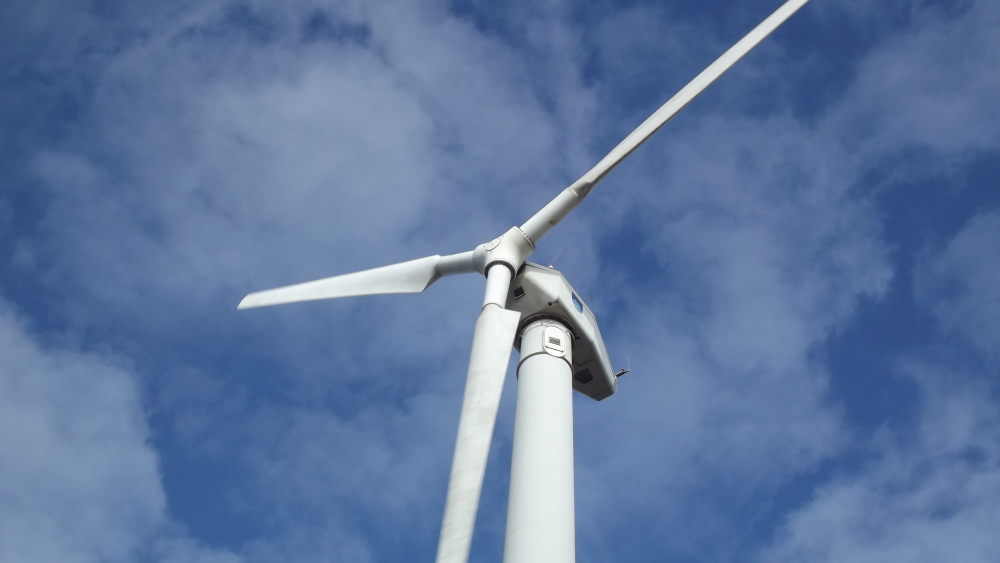
\includegraphics[width=0.48\textwidth]{results/molino.jpg}}
	\quad
	\subfloat[Grayscale image.]{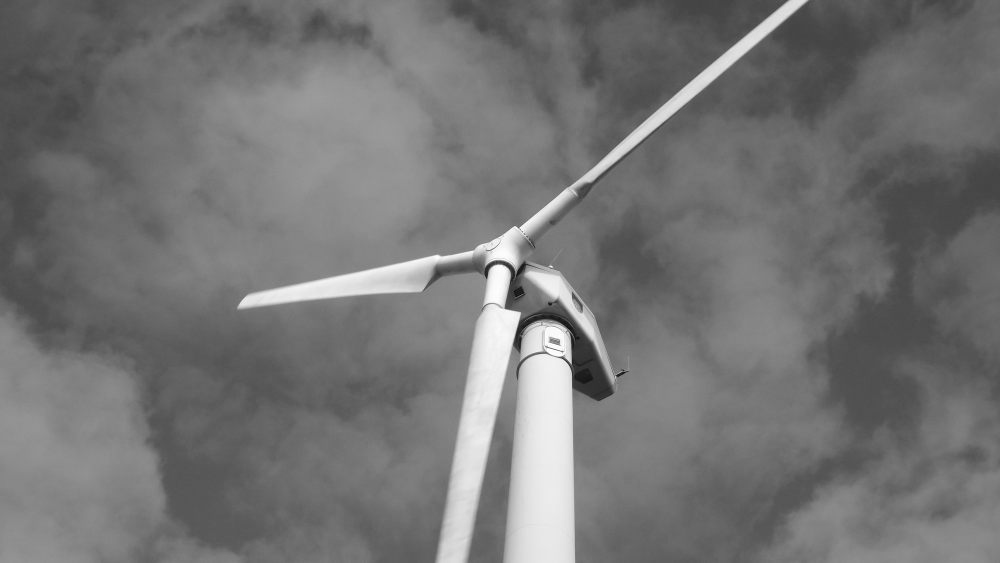
\includegraphics[width=0.48\textwidth]{results/molino_bw.png}}
	\caption{Test image 2: windmill (1000$\times$563 pixels).}
	\label{fig:original2}
\end{figure}

First we show in figures \ref{fig:result2-a} to \ref{fig:result2-c} the results of the first derivative edge detection algorithms. Figures \ref{fig:result2-d} and \ref{fig:result2-e} show the results obtained using the Marr-Hildreth algorithm (both Gaussian and LoG kernels), and figure \ref{fig:result2-f} shows the results obtained using the Haralick algorithm. In table \ref{exectime2} we show the execution time for each one of the algorithms. \\
\begin{figure}[h!]
	\centering
	\subfloat[Roberts.]{\label{fig:result2-a}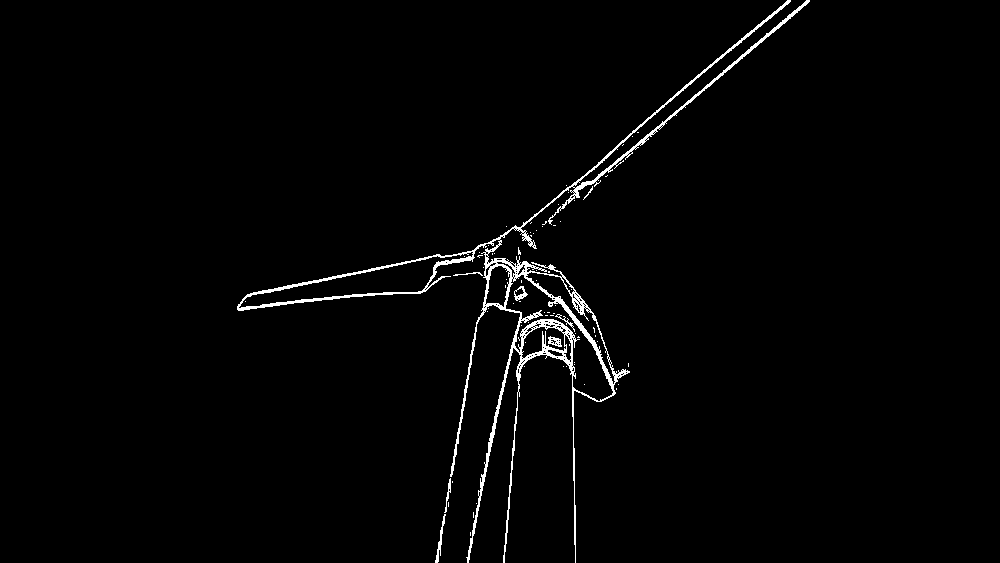
\includegraphics[width=0.42\textwidth]{results/molino_roberts.png}}
	\quad
	\subfloat[Prewitt.]{\label{fig:result2-b}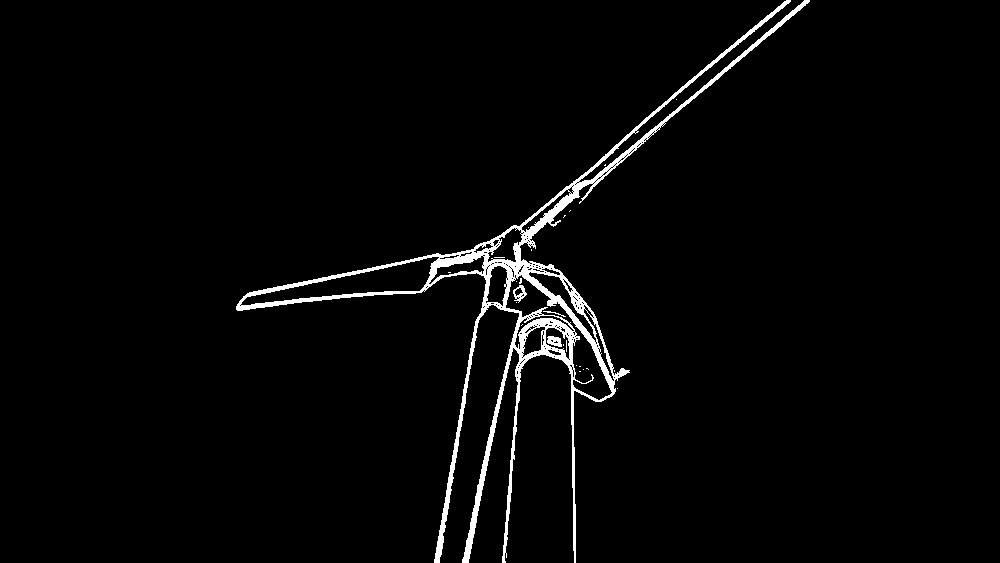
\includegraphics[width=0.42\textwidth]{results/molino_prewitt.png}}
	
	\subfloat[Sobel.]{\label{fig:result2-c}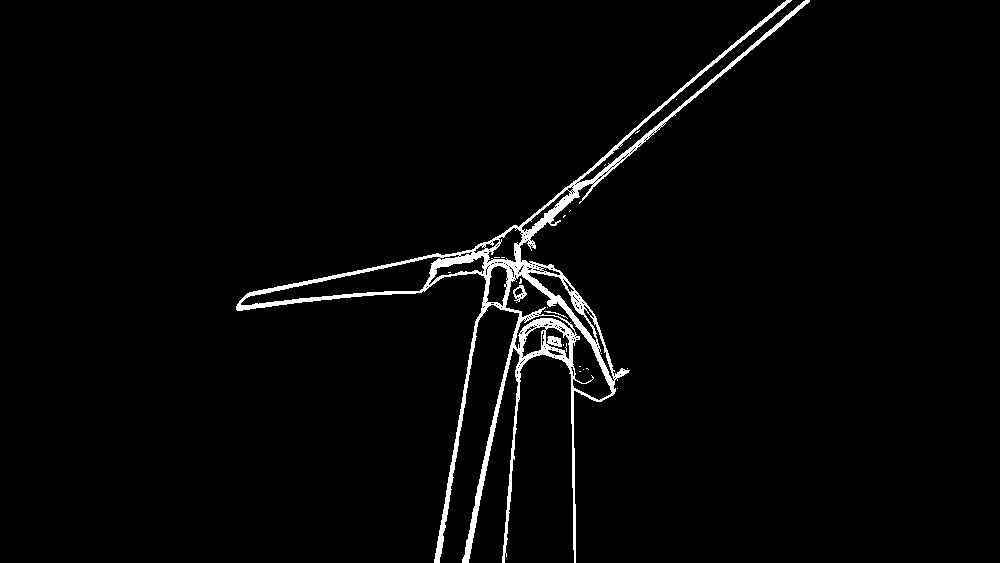
\includegraphics[width=0.42\textwidth]{results/molino_sobel.png}}
	\quad
	\subfloat[Marr-Hildreth (Gaussian).]{\label{fig:result2-d}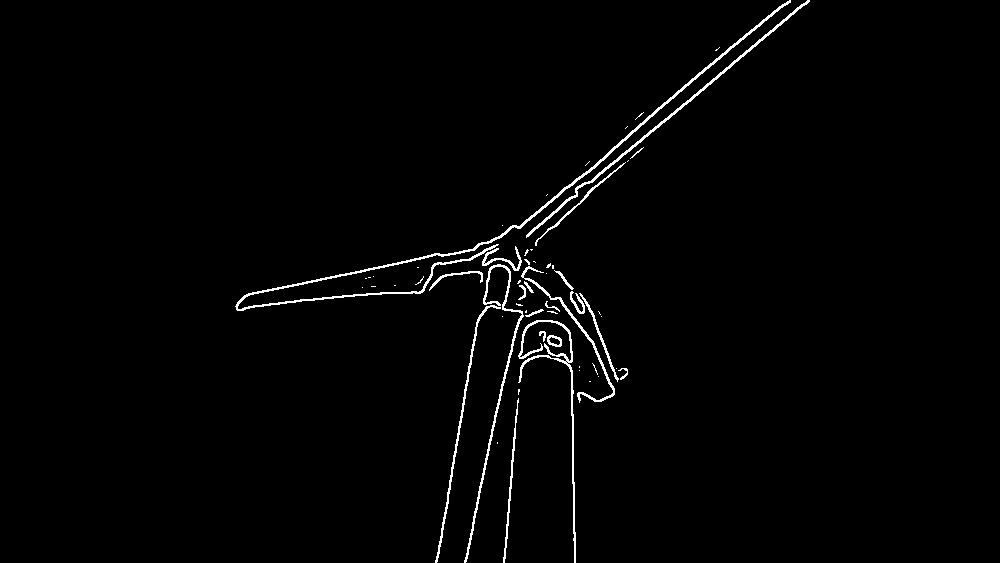
\includegraphics[width=0.42\textwidth]{results/molino_marr-hildreth.png}}

	\subfloat[Marr-Hildreth (LoG).]{\label{fig:result2-e}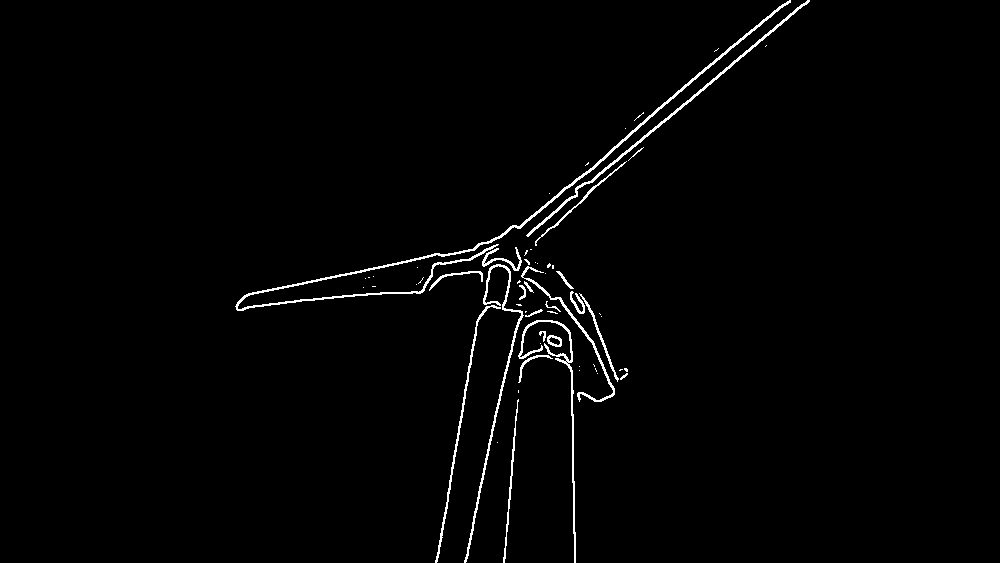
\includegraphics[width=0.42\textwidth]{results/molino_marr-hildreth-log.png}}
	\quad
	\subfloat[Haralick.]{\label{fig:result2-f}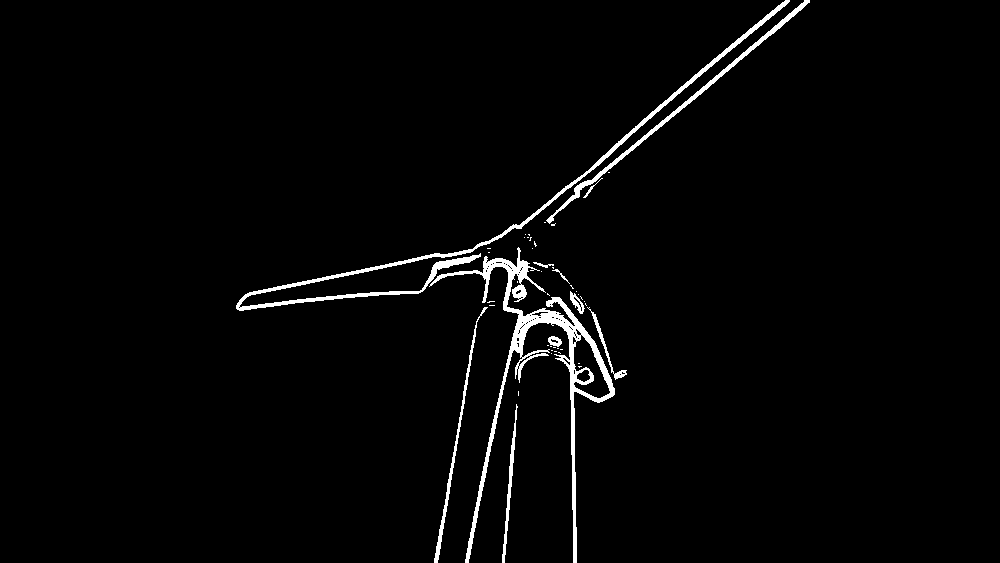
\includegraphics[width=0.42\textwidth]{results/molino_haralick.png}}
	\caption{Results of the first derivative, Marr-Hildreth and Haralick algorithms using the figure \ref{fig:original2} as input image.}
	\label{fig:result2}
\end{figure}

\begin{table}[h!]
	\begin{center}
	\begin{tabular}{| l | r |}
		\hline \rule{0pt}{3ex}
		\cellcolor[gray]{0.8} \textbf{Algorithm}	& \cellcolor[gray]{0.8} \textbf{Execution time (s)}	\\ \hline \rule{0pt}{3ex}
		Roberts, Prewitt and Sobel					& $0.550 \ s$										\\ \hline \rule{0pt}{3ex}
		Marr-Hildreth (Gaussian)					& $1.050 \ s$										\\ \hline \rule{0pt}{3ex}
		Marr-Hildreth (LoG)							& $1.440 \ s$										\\ \hline \rule{0pt}{3ex}
		Haralick									& $0.930 \ s$										\\
		\hline
	\end{tabular}
	\end{center}
	\caption{Execution time of the algorithms using the figure \ref{fig:original2} as input image (1000$\times$563 pixels, 3 channels).}
	\label{exectime2}
\end{table}
\vspace{0.5cm}

It is now visible the difference in performance between the first derivative edge detection algorithms and the second derivative ones. We can see in figure \ref{fig:result3} an area of ​​interest of the image, enlarged to better view of the detail. Note that none of the first derivative methods (even with a loose threshold) detect the lower edge of the blade (which is shaded). Neither Haralick algorithm detects it. However, the Marr-Hildreth algorithm detects it, using either a Gaussian or a LoG kernel. \\

Another observation is that the edges detected by the Haralick algorithm appear to be thicker than those detected with the other algorithms. This may be due the regularity that Haralick assumes, previously mentioned. \\

\begin{figure}[h!]
	\centering
	\subfloat[Original.]{\label{fig:result3-a}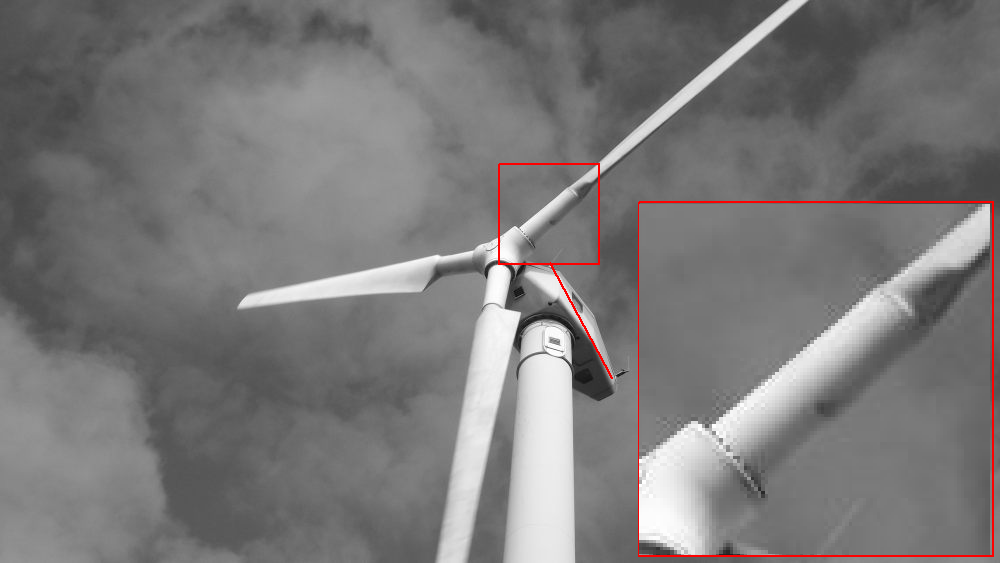
\includegraphics[width=0.48\textwidth]{results/molino_bw_zoom.png}}

	\subfloat[Roberts.]{\label{fig:result3-b}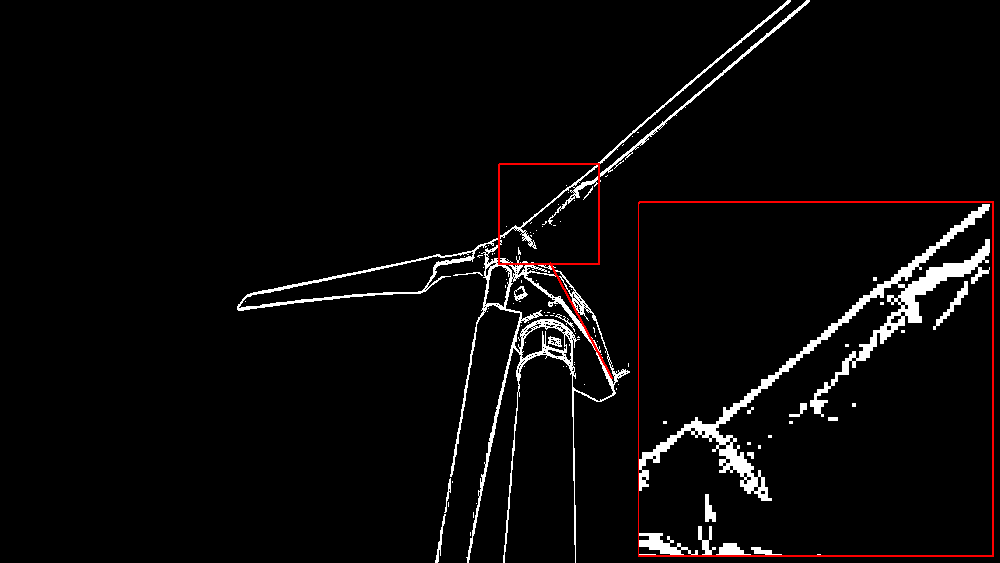
\includegraphics[width=0.48\textwidth]{results/molino_roberts_zoom.png}}
	\quad
	\subfloat[Prewitt.]{\label{fig:result3-c}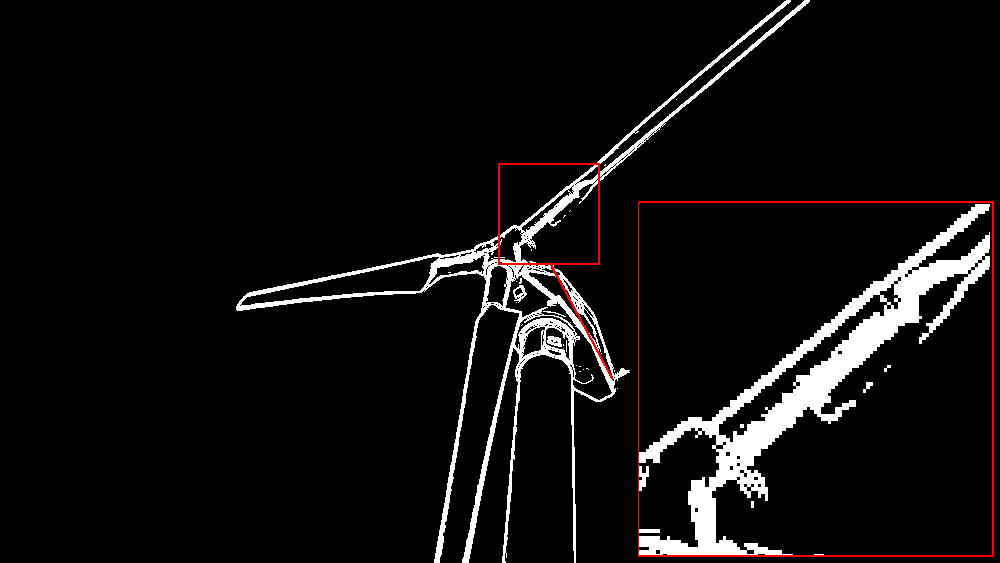
\includegraphics[width=0.48\textwidth]{results/molino_prewitt_zoom.png}}
	
	\subfloat[Sobel.]{\label{fig:result3-d}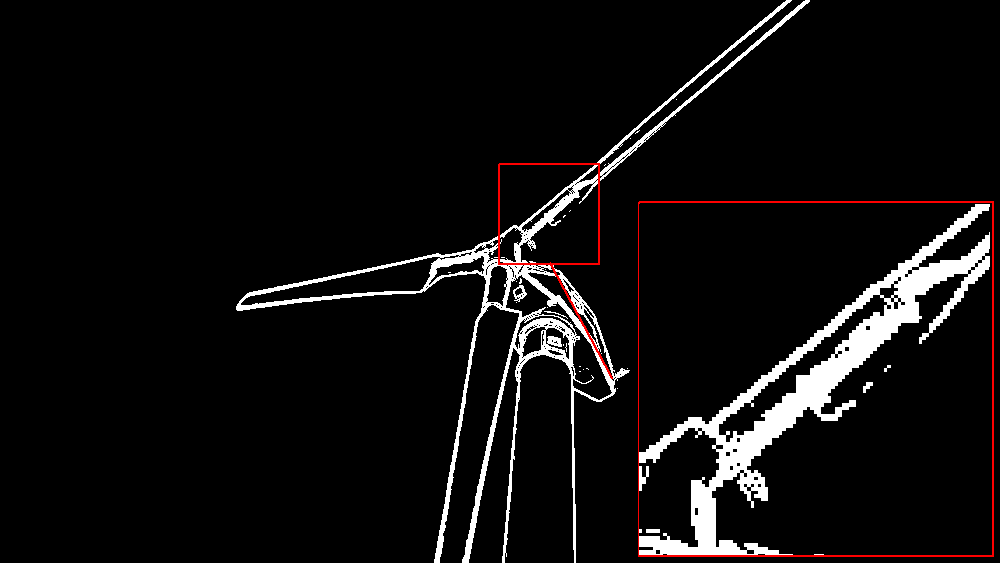
\includegraphics[width=0.48\textwidth]{results/molino_sobel_zoom.png}}
	\quad
	\subfloat[Marr-Hildreth (Gaussian).]{\label{fig:result3-e}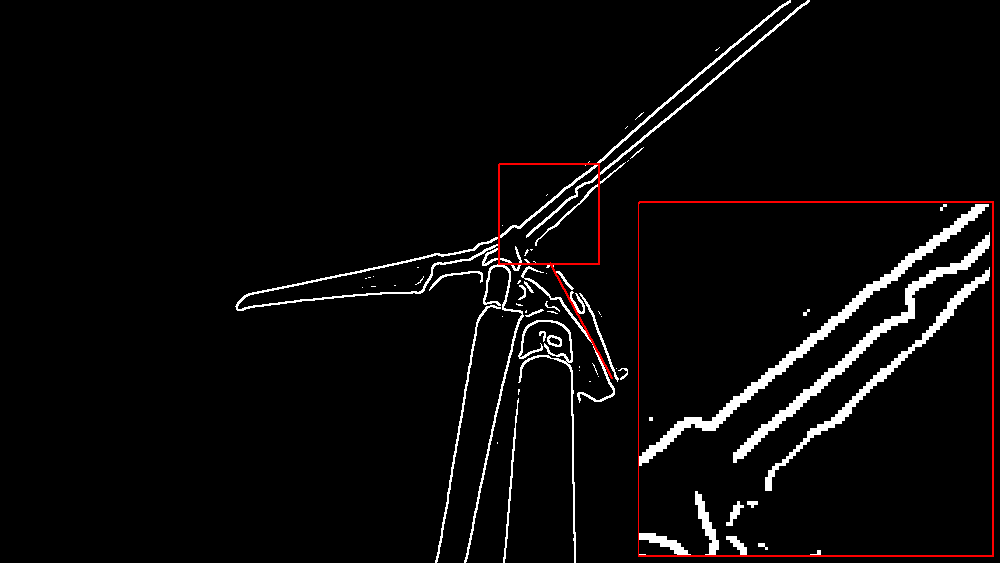
\includegraphics[width=0.48\textwidth]{results/molino_marr-hildreth_zoom.png}}

	\subfloat[Marr-Hildreth (LoG).]{\label{fig:result3-f}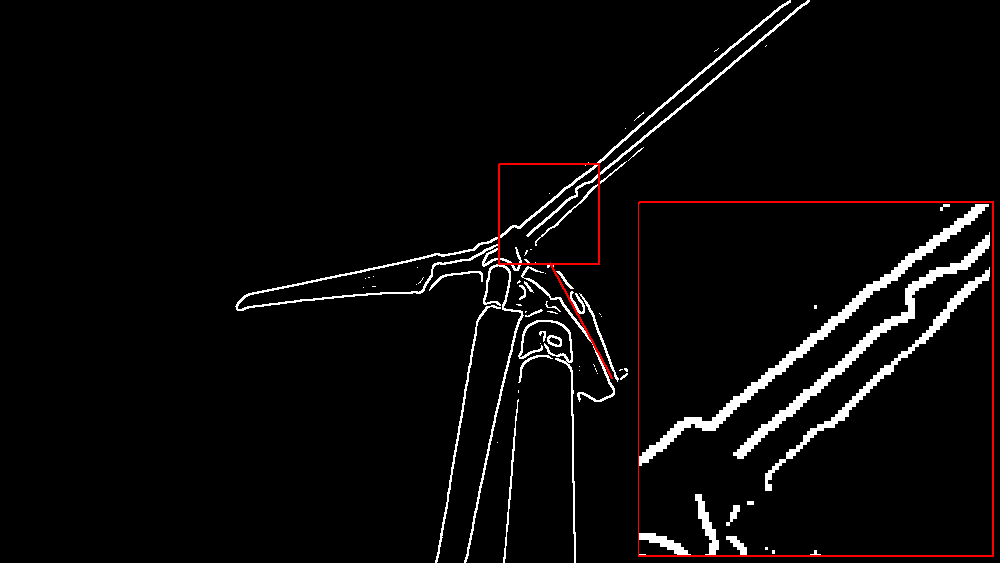
\includegraphics[width=0.48\textwidth]{results/molino_marr-hildreth-log_zoom.png}}
	\quad
	\subfloat[Haralick.]{\label{fig:result3-g}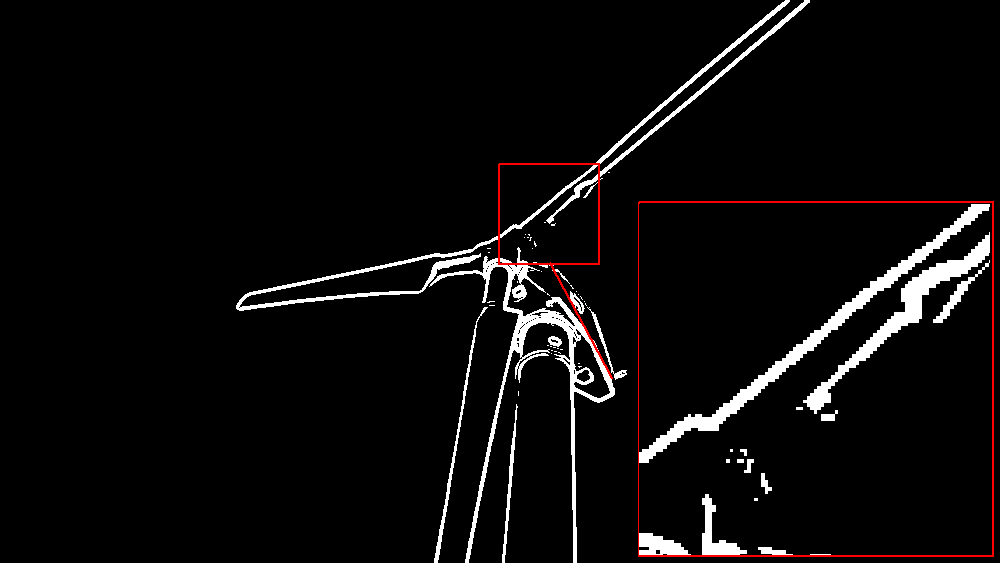
\includegraphics[width=0.48\textwidth]{results/molino_haralick_zoom.png}}
	\caption{Results of the algorithms using the figure \ref{fig:original2} as input image, enlarging an interesting area.}
	\label{fig:result3}
\end{figure}

\clearpage
%-------------------------------------------------------------------------------
\section{Conclusions}
\label{sec:conclusions}

We have discussed and carefully implemented some of the more traditional methods of edge detection in digital images. We have tested the implemented algorithms with synthetic and real images, obtaining generally the expected results, taking into account the limitations of these methods. \\

The first derivative algorithms (Roberts, Prewitt and Sobel) have the advantage of having a very simple implementation. Also they run extremely fast, because they only consists of a convolution with a very small kernel (2$\times$2 or 3$\times$3 pixels). The results obtained with these methods are quite good, considering its simplicity, but they have problems such as noise and discontinuity at the edges. \\

The second derivative algoritms (Marr-Hildreth \& Haralick) involve several more operations, since more convolutions (and with larger kernels) are performed. In real images, they have better behavior towards first derivative algorithms. \\

Comparing the two versions of the Marr-Hildreth algorithm, is significantly faster the version with Gaussian kernel and numerical approximation of the Laplacian. The LoG kernel version, while slower (since it needs a larger kernel to achieve similar results) is more accurate, because it makes no approximation to calculate the Laplacian (it is calculated analytically before creating the kernel). It is also possible to manage the size of the kernel, which represents a scale parameter of the algorithm, being able to obtain a highly detailed edge image using small kernels, or just more noticeable edges using larger kernels. \\

Haralick's algorithm, although it shares the Marr-Hildreth idea of finding zero crossings of the second derivative, has some quite different ideas. It is the only one of these algorithms which works with an approximation of the intensity in the neighborhood of a pixel, using a bicubic polinimial function. This supposes a fairly large regularity in the image, which is not always true, and sometimes leads to detect edges where none of them exist, and get some thicker edges too. \\

All algorithms have their advantages and disadvantages. Choosing one or other may depend on requirements after edge detection. \\ 

% At the end:
Finally, this paper is a summary of some classical edge detection algorithms. In the preparation of this paper, no similar material (concentrated in one text) was found, so this paper appears to be useful material for whom starts studying edge detection methods. \\

\clearpage
%-------------------------------------------------------------------------------
\section{Examples}
\label{sec:examples}

\subsection{Images}

Further examples obtained with the implemented algorithms are shown in figures \ref{fig:example1} and \ref{fig:example2}. More examples can be found in the online \href{http://link_to_demo}{demo}. \\

\begin{figure}[h!]
	\centering
	\subfloat[Original.]{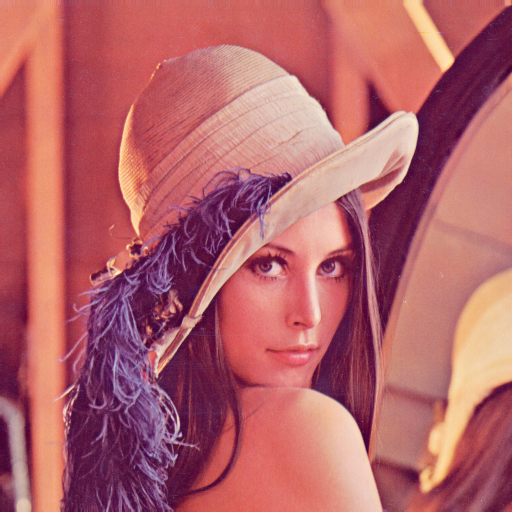
\includegraphics[width=0.3\textwidth]{examples/lena.png}}
	\quad
	\subfloat[Grayscale.]{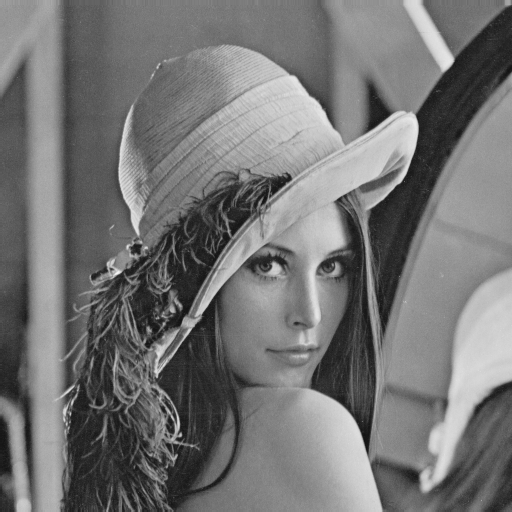
\includegraphics[width=0.3\textwidth]{examples/lena_bw.png}}

	\subfloat[Roberts.]{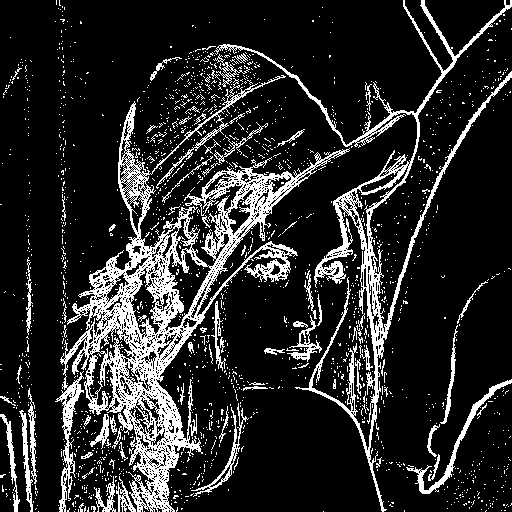
\includegraphics[width=0.3\textwidth]{examples/lena_roberts.png}}
	\quad
	\subfloat[Prewitt.]{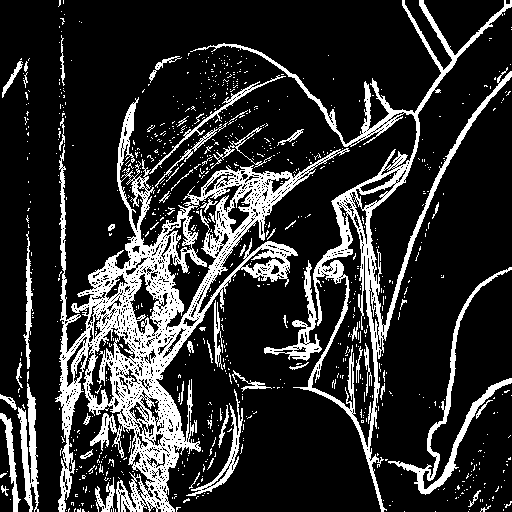
\includegraphics[width=0.3\textwidth]{examples/lena_prewitt.png}}
	\quad
	\subfloat[Sobel.]{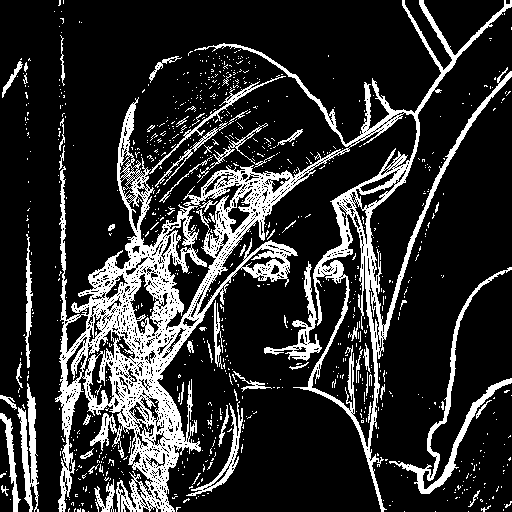
\includegraphics[width=0.3\textwidth]{examples/lena_sobel.png}}

	\subfloat[Marr-Hildreth (Gaussian).]{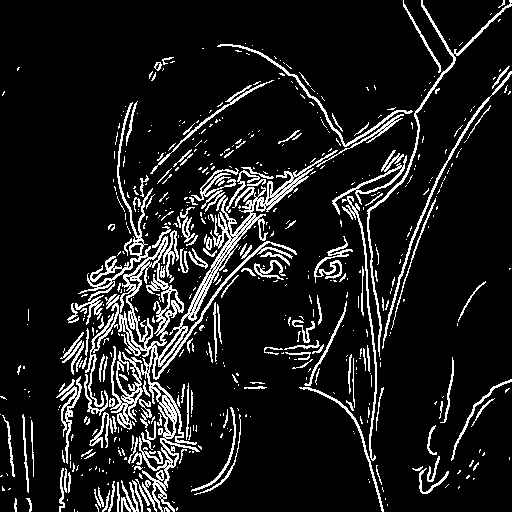
\includegraphics[width=0.3\textwidth]{examples/lena_marr-hildreth.png}}
	\quad
	\subfloat[Marr-Hildreth (LoG).]{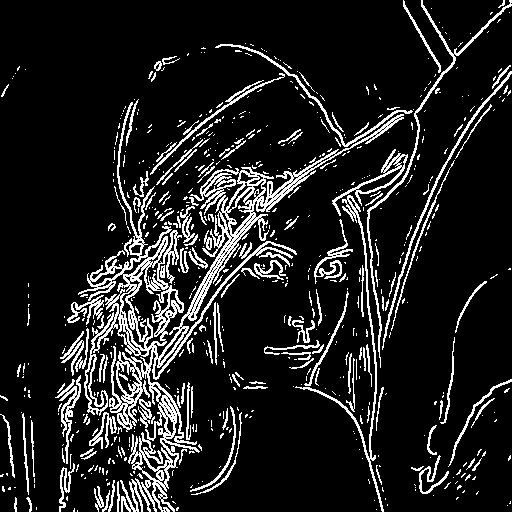
\includegraphics[width=0.3\textwidth]{examples/lena_marr-hildreth-log.png}}
	\quad
	\subfloat[Haralick.]{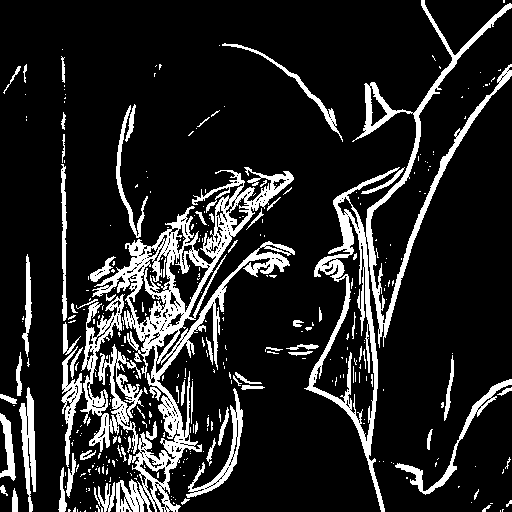
\includegraphics[width=0.3\textwidth]{examples/lena_haralick.png}}
	\caption{Example: Lena (512$\times$512 pixels).}
	\label{fig:example1}
\end{figure}

\begin{figure}[t!]
	\centering
	\subfloat[Original.]{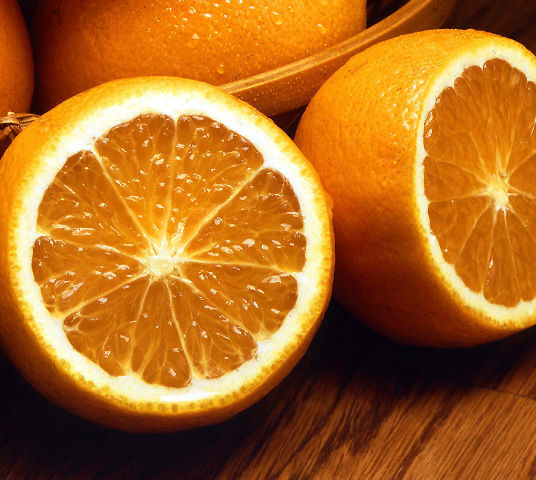
\includegraphics[width=0.3\textwidth]{examples/oranges.png}}
	\quad
	\subfloat[Grayscale.]{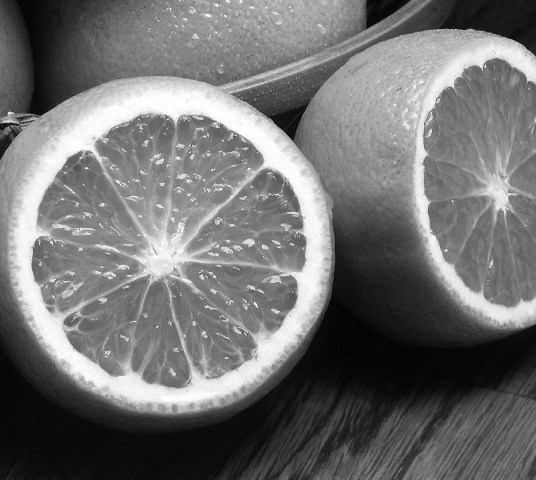
\includegraphics[width=0.3\textwidth]{examples/oranges_bw.png}}

	\subfloat[Roberts.]{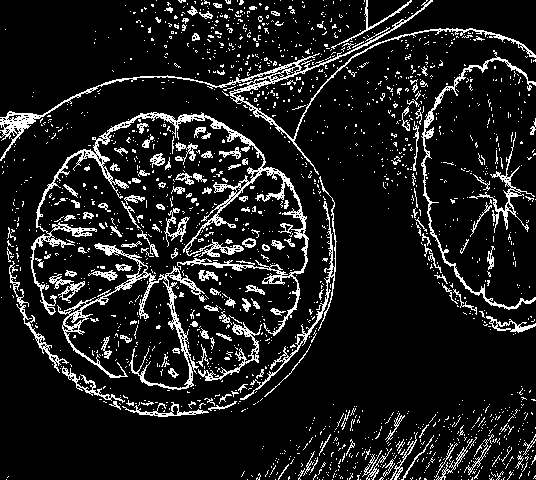
\includegraphics[width=0.3\textwidth]{examples/oranges_roberts.png}}
	\quad
	\subfloat[Prewitt.]{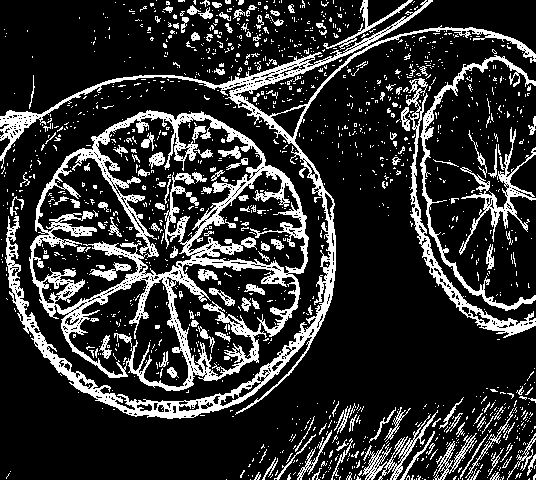
\includegraphics[width=0.3\textwidth]{examples/oranges_prewitt.png}}
	\quad
	\subfloat[Sobel.]{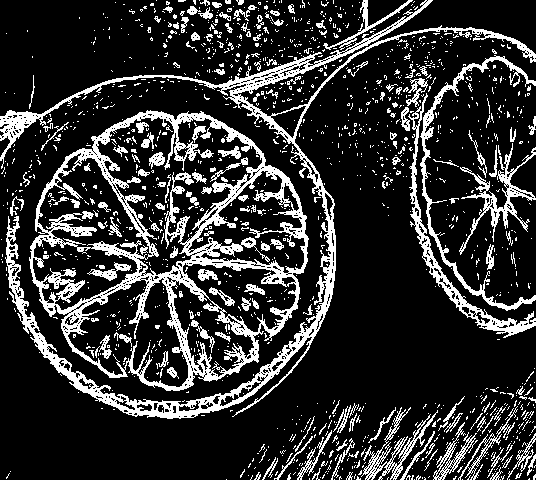
\includegraphics[width=0.3\textwidth]{examples/oranges_sobel.png}}

	\subfloat[Marr-Hildreth (Gaussian).]{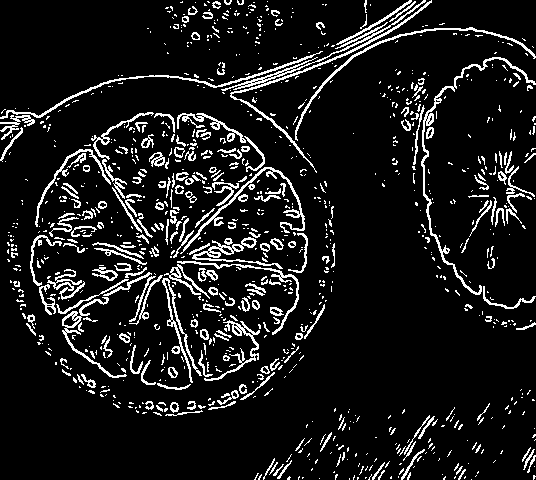
\includegraphics[width=0.3\textwidth]{examples/oranges_marr-hildreth.png}}
	\quad
	\subfloat[Marr-Hildreth (LoG).]{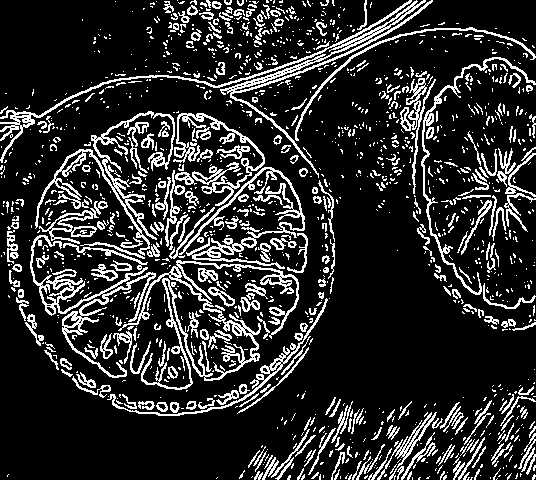
\includegraphics[width=0.3\textwidth]{examples/oranges_marr-hildreth-log.png}}
	\quad
	\subfloat[Haralick.]{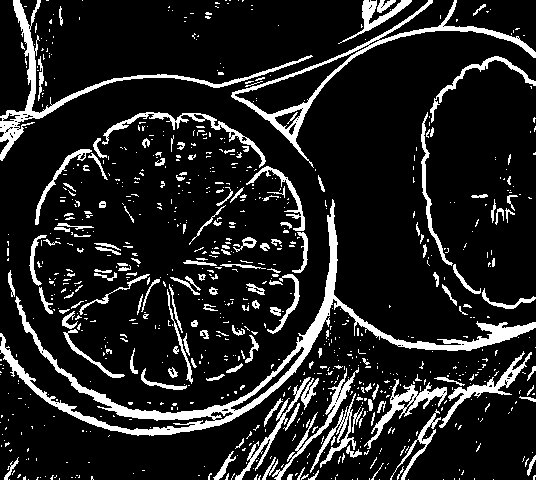
\includegraphics[width=0.3\textwidth]{examples/oranges_haralick.png}}
	\caption{Example: Oranges (536$\times$480 pixels).}
	\label{fig:example2}
\end{figure}

Some observations: 
\begin{itemize}
	\item The first derivative algorithms, although they work properly and quickly, have some problems like discontinuity in the edges. They are also very affected by noise in images, appearing unwanted isolated edges. \\
	\item The Marr-Hildreth algorithm (in its two versions) achieved interesting results in the edge detail. This algorithm provides a first step to regularity in the image, since the filtering with a Gaussian kernel. This behavior can be seen in Lena's hair (figure \ref{fig:example1}), or in the inside of the oranges (example \ref{fig:example2}). \\
	\item As mentioned earlier, Haralick's algorithm is the first to assume greater regularity of the image in the neighborhood of a pixel (third order). This causes thicker edges, as shown in both examples. But, note that some edges are only detected with this algorithm, e.g. the lower edges of the oranges, which are in the shadow, in figure \ref{fig:example2}. These edges are quite smooth, so that the Haralick model is well suited to them, and they do not represent an abrupt change in the intensity to be detected by other methods. \\
\end{itemize}

%\vspace{2cm}

%\begin{figure}[t!]
%	\centering
%	\subfloat[Original.]{\includegraphics[width=0.3\textwidth]{examples/shapes.png}}

%	\subfloat[Roberts.]{\includegraphics[width=0.3\textwidth]{examples/shapes_roberts.png}}
%	\quad
%	\subfloat[Prewitt.]{\includegraphics[width=0.3\textwidth]{examples/shapes_prewitt.png}}
%	\quad
%	\subfloat[Sobel.]{\includegraphics[width=0.3\textwidth]{examples/shapes_sobel.png}}

%	\subfloat[Marr-Hildreth (Gaussian).]{\includegraphics[width=0.3\textwidth]{examples/shapes_marr-hildreth.png}}
%	\quad
%	\subfloat[Marr-Hildreth (LoG).]{\includegraphics[width=0.3\textwidth]{examples/shapes_marr-hildreth-log.png}}
%	\quad
%	\subfloat[Haralick.]{\includegraphics[width=0.3\textwidth]{examples/shapes_haralick.png}}
%	\caption{Example: Shapes.}
%	\label{fig:example3}
%\end{figure}

%-------------------------------------------------------------------------------
\subsection{Video}

%TODO: videos de ejemplo con todos los métodos.

This is an example of applying the edge detection algorithms described here, frame by frame, to a video: 
\begin{itemize}
	\centering
	\item \href{http://iie.fing.edu.uy/~haldos/ipol/video.mov}{original} (xxxMb).
\end{itemize}
\begin{multicols}{2}
\begin{itemize}
	\item \href{http://iie.fing.edu.uy/~haldos/ipol/video-roberts.mov}{roberts version} (xxxMb).
	\item \href{http://iie.fing.edu.uy/~haldos/ipol/video-prewitt.mov}{prewitt version} (xxxMb).
	\item \href{http://iie.fing.edu.uy/~haldos/ipol/video-sobel.mov}{sobel version} (xxxMb).
	\item \href{http://iie.fing.edu.uy/~haldos/ipol/video-marr-hildreth-gaussian.mov}{marr-hildreth-gaussian version} (xxxMb).
	\item \href{http://iie.fing.edu.uy/~haldos/ipol/video-marr-hildreth-log.mov}{marr-hildreth-log version} (xxxMb).
	\item \href{http://iie.fing.edu.uy/~haldos/ipol/video-haralick.mov}{haralick version} (xxxMb).
\end{itemize}
\end{multicols}

%-------------------------------------------------------------------------------
%\begin{thebibliography}{9}
%\end{thebibliography}

\bibliography{bibliography}

\clearpage
%-------------------------------------------------------------------------------
\section{Appendix 1: Common operations}
\label{sec:appendix1}

All algorithms implemented use some common operations that are independent of the algorithms themselves. 
These operations, although basic, have a great impact on the algorithm outcome, and thus they need to be 
implemented with care.\\

\subsection{Grayscale conversion}

The first step in every algorithm presented above is to convert color images to gray intensity images. 
We use the libpng coefficients to do this:
\begin{equation}
    Y = (6968 R + 23434 G + 2366 B) / 32768
\end{equation}
where $R$, $G$ and $B$ are the red, green and blue components respectively.\\

%-------------------------------------------------------------------------------
\subsection{Kernel generation}
\label{sec:appendix2}

Some of the algorithms presented above require the use of a Gaussian kernel or a LoG kernel. These 
kernels are generated by sampling the corresponding analytical function, which in each case depends 
on the parameter $\sigma$ (standard deviation of the Gaussian function). The result is an array of 
size $n$ by $n$.\\

\subsubsection{Gaussian kernel}

We generate the Gaussian kernel by sampling the 2-D Gaussian function\footnote{Note that for simplicity 
we omitted the normalizing coefficient $1/\sqrt{2\pi\sigma^2}$.}
\begin{equation}
	\label{eq:gaussian_function}
	G(x,y) = e^{-\frac{x^2+y^2}{2\sigma^2}}
\end{equation}
where $\sigma$ is the standard deviation (sometimes $\sigma$ is called the \textit{scale space constant}).\\

The size of the kernel $n$ and the standard deviation of the exponential function $\sigma$ are both 
input parameters, but these are not strictly independent of each other. We need a value 
of $n$ large enough to ensure that no information is lost when creating the kernel $G$. To ensure this, we take 
$n$ equal to the first odd integer greater than $6\sigma$. Larger values of $n$ does not add more 
significant samples ​​of $G$, and increases the number of operations in the convolution.\\

Figure \ref{fig:gaussian_kernel} shows a Gaussian kernel, generated with $\sigma = 4$ and $n = 25$ 
(first odd integer greater than $6\sigma=24$).\\

\begin{SCfigure}[][!t]
	\centering
	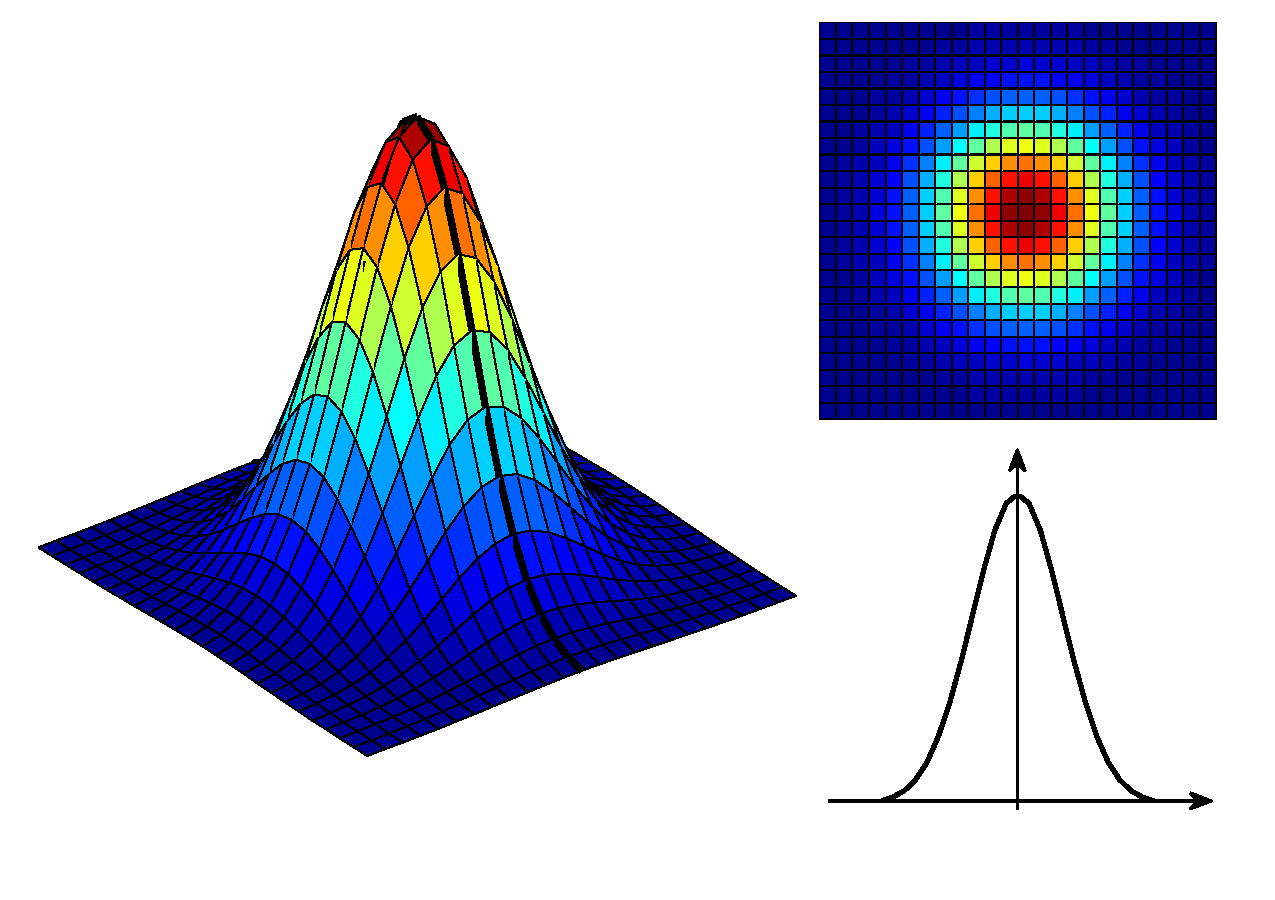
\includegraphics[width=0.5\textwidth]{kernel_gaussian.pdf}
	\caption{Gaussian kernel, $\sigma=4$, $n=25$. Is easy to see that the selected value of n is 
sufficient to have a good approximation of the Gaussian function in the kernel.}
	\label{fig:gaussian_kernel}
\end{SCfigure}

\subsubsection{LoG kernel}

We can obtain analytically the Laplacian of Gaussian $\nabla^2G(x,y)$ first, and generate a kernel 
with the result function. Use this kernel for edge detection involves only one convolution with 
the input image (unlike the case of Gaussian kernel, where we have to make two convolutions, one 
with the kernel and another with the Laplacian operator).\\

\begin{equation}
	LoG \stackrel{\triangle}{=}\nabla^2G(x,y)=\frac{\partial^2}{\partial^2 x}G(x,y) + \frac{\partial^2}{\partial^2 y}G(x,y)
\end{equation}

We first obtain:

\begin{equation} 
	\frac{\partial}{\partial x}G(x,y)=-\frac{x}{\sigma^2}e^{-(x^2+y^2)/2\sigma^2}
\end{equation}

And then:

\begin{equation} 
	\frac{\partial^2}{\partial^2 x}G(x,y)=\frac{x^2-\sigma^2}{\sigma^4}e^{-(x^2+y^2)/2\sigma^2} 
\end{equation}

Similarly:

\begin{equation} 
	\frac{\partial^2}{\partial^2 y}G(x,y)=\frac{y^2-\sigma^2}{\sigma^4}e^{-(x^2+y^2)/2\sigma^2} 
\end{equation}

Therefore we obtain:

\begin{equation}
	\label{eq:log_function}
	LoG(x,y)=\frac{x^2+y^2-2\sigma^2}{\sigma^4}e^{-(x^2+y^2)/2\sigma^2}
\end{equation}\\

Now we generate the LoG kernel by sampling this function. Figure \ref{fig:log_kernel} shows a LoG kernel, generated using the 
values $\sigma=4$ and $n=31$.\\

\begin{SCfigure}[][!t]
	\centering
	\includegraphics[width=0.5\textwidth]{kernel_log.pdf}
	\caption{Laplacian of a Gaussian kernel, $\sigma=4$, $n=31$. The selected value of n is sufficient 
to have a good approximation of the LoG function in the kernel, but is greater than in the case of 
Gaussian kernel.}
	\label{fig:log_kernel}
\end{SCfigure}

\subsubsection{Gaussian and LoG functions comparison}

As we said before, the size of the kernel $n$ and the standard deviation of the exponential function 
$\sigma$ are not independent of each one. This is because the function LoG is "wider" that the 
Gaussian function (i.e. LoG function has a slower decay), so we need a greater value of $n$ to 
generate a correctly sampled LoG kernel than the needed in the case of the Gaussian kernel, with the same $\sigma$.\\

Figure \ref{fig:kernels} shows both functions generated with the same value of $\sigma$. Is clearly 
required a larger kernel size in the case of the LoG function (approximately 18\% more). For 
example, using $\sigma=4$, the optimum value for $n$ in the case of the Gaussian function is the 
first odd integer greater than $6*\sigma$, which is $25$, and for the case of LoG function, would 
be $29$.\\

\begin{SCfigure}[][!t]
	\centering
	\includegraphics[width=0.5\textwidth]{kernels.pdf}
	\caption{Comparison of the Gaussian and LoG functions.}
	\label{fig:kernels}
\end{SCfigure}

\clearpage
%-------------------------------------------------------------------------------
\section{Appendix 2: Implementation}
\label{sec:appendix2}

\subsection{Roberts, Prewitt and Sobel}
% Please do NOT edit this file.
% It has been automatically generated
% by a perl script from the original cxx sources
% in the Insight/Examples directory

% Any changes should be made in the file
% src/test_fded.c


The source code for this section can be found in the file \verb|test_fded.c|.\\  First derivative edge detectors (Roberts, Prewitt and Sobel), main C file.\\
  
  Parameters:
	\begin{itemize}
		\item \texttt{input\_image} - Input image.
		\item \texttt{threshold} - Threshold for gradient image ($0\leq th \leq 1$).
		\item \texttt{padding\_method} - Padding method flag (in convolution): 0 means zero-padding, 1 means image boundary reflection.
	\end{itemize}

	\textit{Note: Output images are saved with the filenames ``\texttt{roberts.png}'', ``\texttt{prewitt.png}'' and ``\texttt{sobel.png}''.} \\

	Includes:
\small
\begin{lstlisting}
	#include "iio.c"
	#include "2dconvolution.c"
	#include <time.h>
\end{lstlisting}
\vspace{1ex}
\normalsize
  Macros:
\small
\begin{lstlisting}
#define MAX(x, y) (((x) > (y)) ? (x) : (y))
#define MIN(x, y) (((x) < (y)) ? (x) : (y))
#define THRESHOLD(x, th) (((x) > (th)) ? (255) : (0))
\end{lstlisting}
\vspace{1ex}
\normalsize
	\vspace{0.5cm}
	\Large{Main function} \\
\small
\begin{lstlisting}
int main(int argc, char *argv[]) {
\end{lstlisting}
\vspace{1ex}
\normalsize
	Load input image (using \textit{iio}): \\
\small
\begin{lstlisting}
		int w, h, pixeldim;
		float *im_orig = iio_read_image_float_vec(argv[1], &w, &h, &pixeldim);
\end{lstlisting}
\vspace{1ex}
\normalsize
	Grayscale conversion (if necessary): explained in \ref{app:marr-hildreth}. \\ \\
	Define the normalized Roberts, Prewitt and Sobel operators: \\
	(We use $3\times 3$ operators)
	\begin{itemize}
		\item	Roberts:
				$$
				R_1 = \begin{bmatrix} -1 & 0 & 0 \\ 0 & 1 & 0 \\ 0 & 0 & 0 \end{bmatrix}
				$$
				$$
				R_2 = \begin{bmatrix} 0 & -1 & 0 \\ 1 & 0 & 0 \\ 0 & 0 & 0 \end{bmatrix}
				$$
		\item	Prewitt:
				$$
				P_1 = \begin{bmatrix} \frac{-1}{6} & \frac{-1}{6} & \frac{-1}{6} \\ 0 & 0 & 0 \\ \frac{1}{6} & \frac{1}{6} & \frac{1}{6} \end{bmatrix}
				$$
				$$
				P_2 = \begin{bmatrix} \frac{-1}{6} & 0 & \frac{1}{6} \\ \frac{-1}{6} & 0 & \frac{1}{6} \\ \frac{-1}{6} & 0 & \frac{1}{6} \end{bmatrix}
				$$
		\item	Sobel:
				$$
				S_1 = \begin{bmatrix} \frac{-1}{8} & \frac{-1}{4} & \frac{-1}{8} \\ 0 & 0 & 0 \\ \frac{1}{8} & \frac{1}{4} & \frac{1}{8} \end{bmatrix}
				$$
				$$
				S_2 = \begin{bmatrix} \frac{-1}{8} & 0 & \frac{1}{8} \\ \frac{-1}{4} & 0 & \frac{1}{4} \\ \frac{-1}{8} & 0 & \frac{1}{8} \end{bmatrix}
				$$
	\end{itemize}
\small
\begin{lstlisting}
		double roberts_1[9] = {-1, 0, 0, 0, 1, 0, 0, 0, 0};		// ROBERTS
		double roberts_2[9] = { 0,-1, 0, 1, 0, 0, 0, 0, 0};		// OPERATORS
		//---------------------------------------------------------------------------------
		double prewitt_1[9] = {-1,-1,-1, 0, 0, 0, 1, 1, 1};		// PREWITT
		double prewitt_2[9] = {-1, 0, 1,-1, 0, 1,-1, 0, 1};		// OPERATORS
		//---------------------------------------------------------------------------------
		double sobel_1[9] = {-1,-2,-1, 0, 0, 0, 1, 2, 1};		// SOBEL
		double sobel_2[9] = {-1, 0, 1,-2, 0, 2,-1, 0, 1};		// OPERATORS
		//---------------------------------------------------------------------------------
		for (z=0;z<9;z++) {										// NORMALIZATION
			roberts_1[z] /= sqrt(2);
			roberts_2[z] /= sqrt(2);
			prewitt_1[z] /= sqrt(6);
			prewitt_2[z] /= sqrt(6);
			sobel_1[z] /= sqrt(12);
			sobel_2[z] /= sqrt(12);
		}
\end{lstlisting}
\vspace{1ex}
\normalsize
	The input image is convolved with the defined operatos, using the \texttt{conv2d} function in \texttt{2dconvolution.c}:
\small
\begin{lstlisting}
		int padding_method = atoi(argv[3]);
		double *im_r1 = conv2d(im, w, h, roberts_1, 3, padding_method);
		double *im_r2 = conv2d(im, w, h, roberts_2, 3, padding_method);
		double *im_p1 = conv2d(im, w, h, prewitt_1, 3, padding_method);
		double *im_p2 = conv2d(im, w, h, prewitt_2, 3, padding_method);
		double *im_s1 = conv2d(im, w, h, sobel_1, 3, padding_method);
		double *im_s2 = conv2d(im, w, h, sobel_2, 3, padding_method);
\end{lstlisting}
\vspace{1ex}
\normalsize
	Allocate memory for final images:
\small
\begin{lstlisting}
		float *im_roberts = malloc(w*h*sizeof(float));
		float *im_prewitt = malloc(w*h*sizeof(float));
		float *im_sobel = malloc(w*h*sizeof(float));
\end{lstlisting}
\vspace{1ex}
\normalsize
	For each method, two images are obtained (one for each operator). Then the gradient magnitude image is constructed using $M=\sqrt{g_x^2+g_y^2}$. \\
	Also the absolute maximum value of the constructed images is computed, for each method. \\
\small
\begin{lstlisting}
		int i,j, fila, col;
		double max_r = 0;
		double max_p = 0;
		double max_s = 0;
		int imax = w*h;
		for (i=0;i<imax;i++){
			fila = (int)(i/w);
			col = i - w*fila + 1;
			fila += 1;
			j = col + (w+2)*fila;
			// Max in each case
			im_roberts[i] = sqrt(im_r1[j]*im_r1[j] + im_r2[j]*im_r2[j]);
			im_prewitt[i] = sqrt(im_p1[j]*im_p1[j] + im_p2[j]*im_p2[j]);
			im_sobel[i] = sqrt(im_s1[j]*im_s1[j] + im_s2[j]*im_s2[j]);
			// Absolute max
			max_r = MAX(max_r,im_roberts[i]);
			max_p = MAX(max_p,im_prewitt[i]);
			max_s = MAX(max_s,im_sobel[i]);
		}
\end{lstlisting}
\vspace{1ex}
\normalsize
	Thresholded images of each method are created, using the THRESHOLD macro: \\
\small
\begin{lstlisting}
		float th = atof(argv[2]);
		for (i=0;i<imax;i++){
			im_roberts[i] = THRESHOLD(im_roberts[i],th*max_r);
			im_prewitt[i] = THRESHOLD(im_prewitt[i],th*max_p);
			im_sobel[i] = THRESHOLD(im_sobel[i],th*max_s);
		}
\end{lstlisting}
\vspace{1ex}
\normalsize
	Save output image (using \textit{iio}): \\
\small
\begin{lstlisting}
		iio_save_image_float_vec("roberts.png", im_roberts, w, h, 1);
		iio_save_image_float_vec("prewitt.png", im_prewitt, w, h, 1);
		iio_save_image_float_vec("sobel.png", im_sobel, w, h, 1);
\end{lstlisting}
\vspace{1ex}
\normalsize


\subsection{Marr-Hildreth}
\label{app:marr-hildreth}
% Please do NOT edit this file.
% It has been automatically generated
% by a perl script from the original cxx sources
% in the Insight/Examples directory

% Any changes should be made in the file
% src/test_mh.c


The source code for this section can be found in the file \verb|test_mh.c|.\\  Marr-Hildreth edge detector, main C file.\\
  
  Parameters:
	\begin{itemize}
		\item \texttt{input\_image} - Input image.
		\item \texttt{sigma} - Standard deviation $\sigma$ of the Gaussian kernel.
		\item \texttt{n} - Size $n$ of the Gaussian kernel ($n\times n$).
		\item \texttt{tzc} - Threshold in the Zero-Crossing calculation ($0\leq t_{zc}\leq 1$).
		\item \texttt{padding\_method} - Padding method flag (in convolution): 0 means zero-padding, 1 means image boundary reflection.
		\item \texttt{output\_image} - Output image (edges).
	\end{itemize}

	Includes:
\small
\begin{lstlisting}
	#include "iio.c"
	#include "gaussian_kernel.c"
	#include "2dconvolution.c"
	#include <time.h>
\end{lstlisting}
\vspace{1ex}
\normalsize
	\vspace{0.5cm}
	\Large{Main function} \\
\small
\begin{lstlisting}
int main(int argc, char *argv[]) {
\end{lstlisting}
\vspace{1ex}
\normalsize
	Load input image (using \textit{iio}): \\
\small
\begin{lstlisting}
		int w, h, pixeldim;
		float *im_orig = iio_read_image_float_vec(argv[1], &w, &h, &pixeldim);
\end{lstlisting}
\vspace{1ex}
\normalsize
	Grayscale conversion (if necessary): \\
	First is allocated the memory for the grayscale image \texttt{im}, with
	the corresponding correct allocation check. Then the number of channels of the image is checked: if
	\texttt{pixeldim}=3, RGB image is assumed and conversion is needed, else, single channel image (grayscale) is assumed and
	no conversion is required.\\
	The computation of the gray intensity from RGB levels is:
	$$
	I = \frac{6968\times (\text{float})R + 23434\times (\text{float})G + 2366\times (\text{float})B}{32768} \\
	$$
  To perform this operation, a cast is made to float on the values ​​$R$, $G$ and $B$ of the original image. This can be slow, 
  but ensures the correct image conversion. \\
  These coefficients also ensure there is no saturation in the calculation, since $\frac{6968\times 255 + 23434\times 255 + 2366\times 255}{32768} = \frac{8355840}{32768} = 255$.
\small
\begin{lstlisting}
		double *im = malloc(w*h*sizeof(double));
		if (im == NULL){
			fprintf(stderr, "Out of memory...\n");
			exit(EXIT_FAILURE);
		}
		int z;
		int zmax = w*h;	
		if (pixeldim==3){
			for(z=0;z<zmax;z++){
				im[z] =  (double)(6968*im_orig[3*z] + 23434*im_orig[3*z + 1] 
													+ 2366*im_orig[3*z + 2])/32768;
			}
			fprintf(stderr, "images converted to grayscale\n");
		} else {
			for(z=0;z<zmax;z++){
				im[z] = (double)im_orig[z];
			}
			fprintf(stderr, "images are already in grayscale\n");
		}
\end{lstlisting}
\vspace{1ex}
\normalsize
	Generate Gaussian kernel using the \texttt{gaussian\_kernel} function in \texttt{gaussian\_kernel.c}: \\
\small
\begin{lstlisting}
		double *kernel = gaussian_kernel(n,sigma);
\end{lstlisting}
\vspace{1ex}
\normalsize
	Smooth input image with the Gaussian kernel previously generated, using the \texttt{conv2d} function in \texttt{2dconvolution.c}: \\
\small
\begin{lstlisting}
		double *im_smoothed = conv2d(im, w, h, kernel, n, padding_method);
\end{lstlisting}
\vspace{1ex}
\normalsize
	Computation of the Laplacian of the smoothed image: \\
	A $3\times 3$ approximation of the laplacian operator is used: \\
	$$
	\begin{bmatrix}
		1 &  1 & 1 \\
		1 & -8 & 1 \\
		1 &  1 & 1 
	\end{bmatrix}
	$$
	Using the \texttt{conv2d} function, the \texttt{laplacian} image is obtained. \\
\small
\begin{lstlisting}
		double operator[9] = {1, 1, 1, 1, -8, 1, 1, 1, 1};
		double *laplacian = conv2d(im_smoothed, w+n-1, h+n-1, operator, 3, padding_method);
\end{lstlisting}
\vspace{1ex}
\normalsize
	Now the maximum absolute value of the \texttt{laplacian} image is calculated. This value is required
	for thresholding in zero-crossing calculation. \\
\small
\begin{lstlisting}
		double max_l = 0;
		int p;
		int pmax = (w+n+1)*(h+n+1);
		for (p=0;p<pmax;p++){
			if (abs(laplacian[p])>max_l){
				max_l = abs(laplacian[p]);
			}
		}
\end{lstlisting}
\vspace{1ex}
\normalsize
	Zero-crossing: \\
	The image is explored, looking in every pixel a change of sign between neighboring opposite pixels.
 	In every pixel $p$ the funcion \texttt{get\_neighborhood} (in \texttt{2dconvolution.c}) is used to get the
	9 pixels of its neighborhood:
	$$
	\begin{bmatrix}
		p_{up,left}		& p_{up,middle}		& p_{up,right}		\\
		p_{middle,left}	& p					& p_{middle,right}	\\
		p_{down,left}	& p_{down,middle}	& p_{down,right}	
	\end{bmatrix}
	$$
	Then the pixel $p$ is marked as edge pixel if it occurs that:
	\begin{itemize}
	\item $sign(p_{up,left}) \neq sign(p_{down,right})$, or 
	\item $sign(p_{up,middle}) \neq sign(p_{down,middle})$, or 
	\item $sign(p_{up,right}) \neq sign(p_{down,left})$, or
	\item $sign(p_{middle,left}) \neq sign(p_{middle,right})$. \\
	\end{itemize}
\small
\begin{lstlisting}
		float *zero_cross = calloc(w*h,sizeof(float));		
						// this image will only content values 0 and 255
						// but float type is used for saving using iio.
		if (zero_cross == NULL){
			fprintf(stderr, "Out of memory...\n");
			exit(EXIT_FAILURE);
		}
		int ind_en_lapl, fila, col;
		int *offsets = get_neighbors_offset(w+n+1, 3);
		pmax = w*h;
		int dif_fila_col = (n+1)/2;
		for (p=0;p<pmax;p++){
			fila = ((int)(p/w));
			col = p-(w*fila) + dif_fila_col;
			fila += dif_fila_col;
			ind_en_lapl = col + (w+n+1)*fila;
			double *n3 = get_neighborhood(laplacian, ind_en_lapl, 3, offsets);
			if ((n3[3]*n3[5]<0)&&(abs(n3[3]-n3[5])>(tzc*max_l))) {
				// horizontal sign change
				zero_cross[p] = 255;
			} else if ((n3[1]*n3[7]<0)&&(abs(n3[1]-n3[7])>(tzc*max_l))) {
					// vertical sign change
					zero_cross[p] = 255;
				} else if ((n3[2]*n3[6]<0)&&(abs(n3[2]-n3[6])>(tzc*max_l))) {
						// +45deg sign change
						zero_cross[p] = 255;
					} else if ((n3[0]*n3[8]<0)&&(abs(n3[0]-n3[8])>(tzc*max_l))) {
							// -45deg sign change
							zero_cross[p] = 255;
						}
			free_neighborhood(n3);
		}
		free_neighbors_offsets(offsets);
\end{lstlisting}
\vspace{1ex}
\normalsize
	Save output image (using \textit{iio}): \\
\small
\begin{lstlisting}
		iio_save_image_float_vec(argv[6], zero_cross, w, h, 1);
\end{lstlisting}
\vspace{1ex}
\normalsize
	\textit{Note: the main function in \texttt{test\_mh\_log.c} is essentially the same. The only difference is that a LoG kernel is generated (instead of a Gaussian kernel) using the
	\texttt{LoG\_kernel} function in \texttt{gaussian\_kernel.c}. Therefore there is no need to use the laplacian operator, so only one convolution is made.} \\


\subsection{Haralick}
% Please do NOT edit this file.
% It has been automatically generated
% by a perl script from the original cxx sources
% in the Insight/Examples directory

% Any changes should be made in the file
% src/test_haralick.c


The source code for this section can be found in the file \verb|test_haralick.c|.\\  Haralick edge detectors, main C file.\\
  
  Parameters:
	\begin{itemize}
		\item \texttt{input\_image} - Input image.
		\item \texttt{rhozero} - Threshold for the Haralick condition $|\frac{C_2}{2C_3}|\leq\rho_0$.
		\item \texttt{padding\_method} - Padding method flag (in convolution): 0 means zero-padding, 1 means image boundary reflection.
		\item \texttt{output\_image} - Output image (edges).
	\end{itemize}

	Includes:
\small
\begin{lstlisting}
	#include "iio.c"
	#include "2dconvolution.c"
	#include <time.h>
\end{lstlisting}
\vspace{1ex}
\normalsize
	\vspace{0.5cm}
	\Large{Main function} \\
\small
\begin{lstlisting}
int main(int argc, char *argv[]) {
\end{lstlisting}
\vspace{1ex}
\normalsize
	Load input image (using \textit{iio}): \\
\small
\begin{lstlisting}
		int w, h, pixeldim;
		float *im_orig = iio_read_image_float_vec(argv[1], &w, &h, &pixeldim);
\end{lstlisting}
\vspace{1ex}
\normalsize
	Grayscale conversion (if necessary): explained in \ref{app:marr-hildreth}. \\ \\
	Masks calculated by 2-d fitting (using LS) with the function: 
	$$
	f(x,y) = k_1 + k_2x + k_3y + k_4x^2 + k_5xy + k_6*y^2 + k_7x^3 + k_8x^2y + k_9xy^2 + k_{10}y^3 \\
	$$
\small
\begin{lstlisting}
		double masks[10][25] = { {   425,   275,  225,  275,  425,   
									 275,   125,   75,  125,  275,   
                                     225,    75,   25,   75,  225,   
									 275,   125,   75,  125,  275,   
									 425,   275,  225,  275,  425},
								 { -2260,  -620,    0,  620,  2260, 
								   -1660,  -320,    0,  320,  1660, 
								   -1460,  -220,    0,  220,  1460,
                                   -1660,  -320,    0,  320,  1660, 
                                   -2260,  -620,    0,  620, 2260},
								// matrix continues, too large to display in documentation.
\end{lstlisting}
\vspace{1ex}
\normalsize
	Initialise edge image using \texttt{calloc}:
\small
\begin{lstlisting}
		float *edges = calloc(w*h,sizeof(float));
\end{lstlisting}
\vspace{1ex}
\normalsize
	Padding: a larger auxiliary image \texttt{aux} is required to compute the coefficients $k_1$ to $k_{10}$ in every pixel of the original image. \\
	Two different methods are implemented: zero-padding (\texttt{padding\_method}$=0$) and reflection of original image (\texttt{padding\_method}$=1$).
\small
\begin{lstlisting}
		int wx = (w+8);
		int hx = (h+8);
		double *aux = calloc(wx*hx,sizeof(double));
		int fila,col;
		int imax = wx*hx;
		if (padding_method == 0) {
			for(i=0;i<imax;i++){
				fila = (int)(i/wx);
				col = i-(wx*fila);	
				if ( (fila>=4)&&(col>=4)&&(fila<h+4)&&(col<w+4) ) {
					aux[i] = im[(col-4)+(w*(fila-4))];
				}
			}
		}
\end{lstlisting}
\vspace{1ex}
\normalsize
\small
\begin{lstlisting}
		if (padding_method == 1) {
			int fila_refl, col_refl;
			for(i=0;i<imax;i++){
				fila = (int)(i/wx);
				col = i-(wx*fila);
				if (fila<4) {
					fila_refl = 7 - fila;
					if (col<4) { //zone1
						col_refl = 7 - col;
					} else if (col<w+4) {	//zone2
						col_refl = col;
					} else { //zone3
						col_refl = 2*w + 7 - col;
					}
				} else if (fila<h+4) {
					fila_refl = fila;
					if (col<4) { //zone4
						col_refl = 7 - col;
					} else if (col<w+4) { //image
						col_refl = col;
					} else { //zone5
						col_refl =  2*w + 7 - col;
					}
				} else {
					fila_refl = 2*h + 7 - fila;
					if (col<4) { //zone6
						col_refl =	7 - col;
					} else if (col<w+4) {	//zone7
						col_refl = col;
					} else { //zone8
						col_refl =  2*w + 7 - col;
					}
				}
				aux[i] = im[(col_refl-4)+(w*(fila_refl-4))];
			} //for
		}
\end{lstlisting}
\vspace{1ex}
\normalsize
	Haralick algorithm: coefficients $k_1$ to $k_{10}$ are computed in every pixel of the original image 
	(using the function \texttt{get\_neighbors\_offset} to get the index offsets of the neighbor pixels and 
	the function \texttt{get\_neighborhood} to get the neighborhood of a pixel using those index offsets). 
	Once the coefficients are calculated, are computed
	$$
	C_2 = \frac{k_2^2k_4 + k_2k_3k_5 + k_3^2k_6}{k_2^2 + k_3^2}
	$$
	and
	$$
	C_3 = \frac{k_2^3k_7 + k_2^2k_3k_8 + k_2k_3^2k_9 + k_3^3k_{10}}{(\sqrt{k_2^2 + k_3^2})^3},
	$$
	and then the edge condition is evaluated in every pixel; $|\frac{C_2}{2C_3}|\leq\rho_0$. \\
\small
\begin{lstlisting}
		int i_zp, u, v, num_edges;
		num_edges = 0;
		double k[10];
		int *offsets = get_neighbors_offset(wx, 5);
		double acum;
		double C2, C3, denom, sintheta, costheta;
		for(fila=0;fila<h;fila++){
			for(col=0;col<w;col++){
				i = col + w*fila;				// original image & edges image index
				i_zp = (col+4) + wx*(fila+4);	// padded image index
				double *neighborhood = get_neighborhood(aux, i_zp, 5, offsets);
				// k1 to k10 (note: k1 (u=0) is not necessary)
				for(u=0;u<10;u++){
					acum = 0;
					for(v=0;v<25;v++){
						acum += neighborhood[v]*masks[u][v];
					}
					k[u] = acum;
				}
				// compute C2 and C3
				denom = sqrt( k[1]*k[1] + k[2]*k[2] );
				sintheta = - k[1] / denom;
				costheta = - k[2] / denom;
				C2 = k[3]*sintheta*sintheta + k[4]*sintheta*costheta + k[5]*costheta*costheta;
				C3 = k[6]*sintheta*sintheta*sintheta + k[7]*sintheta*sintheta*costheta +
					 k[8]*sintheta*costheta*costheta + k[9]*costheta*costheta*costheta;
				//if ((fabs(C2 / (3*C3))<=rhozero)&&(C3<=0)) {
				if ((fabs(C2 / (3*C3))<=rhozero)) {
					edges[i] = 255;
					num_edges += 1;
				}
				// free neighborhood
				free_neighborhood(neighborhood);
			}
		}
\end{lstlisting}
\vspace{1ex}
\normalsize
	Save output image (using \textit{iio}): \\
\small
\begin{lstlisting}
		iio_save_image_float_vec(argv[4], edges, w, h, 1);
\end{lstlisting}
\vspace{1ex}
\normalsize


\subsection{Gaussian kernel generation}
% Please do NOT edit this file.
% It has been automatically generated
% by a perl script from the original cxx sources
% in the Insight/Examples directory

% Any changes should be made in the file
% src/gaussian_kernel.c


The source code for this section can be found in the file \verb|gaussian_kernel.c|.\\	This file implements the necessary functions for generating 
	Gaussian and LoG (Laplacian of a Gaussian) kernels. It is also 
	done here the alloc and free of the memory needed. \\

	Includes:
\small
\begin{lstlisting}
	#include <math.h> // exp
	#include <stdlib.h> // malloc, calloc, free
	#include <stdio.h> // fprintf
\end{lstlisting}
\vspace{1ex}
\normalsize
	\vspace{0.5cm}
	\Large{Function \texttt{gaussian\_kernel}} \\
 
	\normalsize
	This function generates a Gaussian kernel of size $n\times n$ and standard deviation $\sigma$. \\
\small
\begin{lstlisting}
double *gaussian_kernel(int n, float sigma){
\end{lstlisting}
\vspace{1ex}
\normalsize
	Memory allocation for the kernel: \\
\small
\begin{lstlisting}
	double *kernel = malloc(n*n*sizeof(double));
\end{lstlisting}
\vspace{1ex}
\normalsize
	A normalized Gaussian kernel is generated using the expression $e^{-\frac{x^2+y^2}{2\sigma^2}}$. \\
\small
\begin{lstlisting}
	int i;
	int fila, col, x, y;
	double suma = 0;
	int imax = n*n;
	for(i=0;i<imax;i++){
		fila = (int)(i/n);
		col = i-(n*fila);
		y = ((int)(n/2))-fila;
		x = col-((int)(n/2));
		kernel[i] = exp(-(x*x + y*y)/(2*sigma*sigma));
		suma += kernel[i];
	}
\end{lstlisting}
\vspace{1ex}
\normalsize
	Kernel normalization, using the sum of its components. \\
\small
\begin{lstlisting}
	for(i=0;i<n*n;i++){
		kernel[i] = kernel[i]/suma;
	}
\end{lstlisting}
\vspace{1ex}
\normalsize
	Return: \\
\small
\begin{lstlisting}
	return kernel;
\end{lstlisting}
\vspace{1ex}
\normalsize
	\vspace{0.5cm}
	\Large{Function \texttt{free\_gaussian\_kernel}} \\
 
	\normalsize
	This function frees the memory allocated in the function \texttt{gaussian\_kernel}. It receives as parameter the pointer to the array to be freed. \\
\small
\begin{lstlisting}
void free_gaussian_kernel(double* kernel){
\end{lstlisting}
\vspace{1ex}
\normalsize
	Free memory: \\
\small
\begin{lstlisting}
	free(kernel);
\end{lstlisting}
\vspace{1ex}
\normalsize
	\vspace{0.5cm}
	\Large{Function \texttt{LoG\_kernel}} \\
 
	\normalsize
	This function generates a Laplacian of a Gaussian kernel (LoG kernel) of size $n\times n$ and standard deviation $\sigma$. \\
\small
\begin{lstlisting}
double *LoG_kernel(int n, float sigma){
\end{lstlisting}
\vspace{1ex}
\normalsize
	Memory allocation for the kernel: \\
\small
\begin{lstlisting}
	double *kernel = malloc(n*n*sizeof(double));
\end{lstlisting}
\vspace{1ex}
\normalsize
	We generate a Laplacian of a Gaussian kernel using the expression $\frac{x^2 + y^2 - 2\sigma^2}{\sigma^4}e^{-\frac{x^2+y^2}{2\sigma^2}}$. \\
\small
\begin{lstlisting}
	int i;
	int fila, col, x, y;
	double suma = 0;
	int imax = n*n;
	for(i=0;i<imax;i++){
		fila = (int)(i/n);
		col = i-(n*fila);
		y = ((int)(n/2))-fila;
		x = col-((int)(n/2));
		kernel[i] = ( (x*x + y*y - 2*sigma*sigma)/(sigma*sigma*sigma*sigma) )
					*exp(-(x*x + y*y)/(2*sigma*sigma));
	}
\end{lstlisting}
\vspace{1ex}
\normalsize
	Return: \\
\small
\begin{lstlisting}
	return kernel;
\end{lstlisting}
\vspace{1ex}
\normalsize


\subsection{2D convolution}
% Please do NOT edit this file.
% It has been automatically generated
% by a perl script from the original cxx sources
% in the Insight/Examples directory

% Any changes should be made in the file
% src/2dconvolution.c


The source code for this section can be found in the file \verb|2dconvolution.c|.\\  This file contains the necessary functions to compute the convolution between an 
  input array and a kernel (usually the input array is larger than the kernel). \\

	Includes:
\small
\begin{lstlisting}
	#include <stdlib.h> // malloc, calloc, free
	#include <stdio.h> // fprintf
\end{lstlisting}
\vspace{1ex}
\normalsize
	\vspace{0.5cm}
	\Large{Function \texttt{free\_gaussian\_kernel}} \\
 
	\normalsize
	This function frees the memory allocated in the function \texttt{get\_neighborhood}. It receives as parameter the pointer to the array to be freed. \\
\small
\begin{lstlisting}
void free_neighborhood(double* neighborhood){
\end{lstlisting}
\vspace{1ex}
\normalsize
	Free memory: \\
\small
\begin{lstlisting}
	free(neighborhood);
\end{lstlisting}
\vspace{1ex}
\normalsize
	\vspace{0.5cm}
	\Large{Function \texttt{free\_gaussian\_kernel}} \\
 
	\normalsize
	This function frees the memory allocated in the function \texttt{get\_neighbors\_offset}. It receives as parameter the pointer to the array to be freed. \\
\small
\begin{lstlisting}
void free_neighbors_offsets(int* offsets){
\end{lstlisting}
\vspace{1ex}
\normalsize
	Free memory: \\
\small
\begin{lstlisting}
	free(offsets);
\end{lstlisting}
\vspace{1ex}
\normalsize
	\vspace{0.5cm}
	\Large{Function \texttt{get\_neighbors\_offset}} \\
 
	\normalsize
	This function computes the linear array index offsets required to access the neighbor pixels in 
	a neighborhood of size $n\times n$. This computation requires to know the width $w$ of the image. \\
\small
\begin{lstlisting}
int *get_neighbors_offset(int w, int n){
\end{lstlisting}
\vspace{1ex}
\normalsize
	Memory allocation for the index offsets array: \\
\small
\begin{lstlisting}
	int *aux = malloc(n*n*sizeof(int));
\end{lstlisting}
\vspace{1ex}
\normalsize
	Computation of the index offsets array: \\
\small
\begin{lstlisting}
	int imax = n*n;
	int dif_fila_col = (n-1)/2;
	for (i=0;i<imax;i++){
		delta_fila = (int)(i/n)-dif_fila_col;
		delta_col = i-n*((int)(i/n))-dif_fila_col;
		aux[i] = delta_fila*w+delta_col;
	}
\end{lstlisting}
\vspace{1ex}
\normalsize
	Return: \\
\small
\begin{lstlisting}
	return aux;
\end{lstlisting}
\vspace{1ex}
\normalsize
	\vspace{0.5cm}
	\Large{Function \texttt{get\_neighborhood}} \\
 
	\normalsize
	This function returns an array of size $n\times n$ containing the neighbors of the 
  pixel at the position \texttt{pos} of the image \texttt{im}. For this calculation, 
	the index offsets array calculated with the function \texttt{get\_neighbors\_offset} 
	is needed.
\small
\begin{lstlisting}
double *get_neighborhood(double *im, int pos, int n, int* offsets){
\end{lstlisting}
\vspace{1ex}
\normalsize
	Memory allocation for the neighborhood array: \\
\small
\begin{lstlisting}
	double *aux = malloc(n*n*sizeof(double));
\end{lstlisting}
\vspace{1ex}
\normalsize
	Assigning values ​​of the neighborhood: \\
\small
\begin{lstlisting}
	int i;
	int imax = n*n;
	for (i=0;i<imax;i++){
		aux[i] = im[pos+offsets[i]];
	}
\end{lstlisting}
\vspace{1ex}
\normalsize
	Return: \\
\small
\begin{lstlisting}
	return aux;
\end{lstlisting}
\vspace{1ex}
\normalsize
	\vspace{0.5cm}
	\Large{Function \texttt{conv2d}} \\
 
	\normalsize
	This function calculates the convolution of image \texttt{input} (size $w\times h$) with the kernel \texttt{kernel} (size $n\times n$).
	Returns an image of size $(w+n-1)\times(h+n-1)$ (due to padding). The integer \texttt{padding\_method} manages the padding method: $0$
  means zero-padding, $1$ means image boundary reflection. \\
\small
\begin{lstlisting}
double *conv2d(double *input, int w, int h, double *kernel, int n, int padding_method){
\end{lstlisting}
\vspace{1ex}
\normalsize
	Zero padding: reserve memory for an array of size $(w+2(n-1))\times(h+2(n-1))$. \\
\small
\begin{lstlisting}
	int wx = (w+2*(n-1));
	int hx = (h+2*(n-1));
	double *aux = calloc(wx*hx,sizeof(double));
\end{lstlisting}
\vspace{1ex}
\normalsize
	Fill in the values ​​of the image \texttt{aux}, centering the original image \texttt{input} on it (zero-padding). \\
\small
\begin{lstlisting}
	int i,j,fila,col;
	int imax = wx*hx;
	if (padding_method == 0) {
		for(i=0;i<imax;i++){
			fila = (int)(i/wx);
			col = i-(wx*fila);
			if ( (fila>=n-1)&&(col>=n-1)&&(fila<h+n-1)&&(col<w+n-1) ) {
				aux[i] = input[(col-n+1)+(w*(fila-n+1))];
			}
		}
	}
\end{lstlisting}
\vspace{1ex}
\normalsize
 Other padding method: reflection of the image (if \texttt{padding\_method} equal to $1$). \\
\small
\begin{lstlisting}
	if (padding_method == 1) {
		int fila_refl, col_refl;
		for(i=0;i<imax;i++){
			fila = (int)(i/wx);
			col = i-(wx*fila);
			if (fila<n-1) {
				fila_refl = 2*n - 3 - fila;
				if (col<n-1) { //zone1
					col_refl = 2*n - 3 - col;
				} else if (col<w+n-1) {	//zone2
					col_refl = col;
				} else { //zone3
					col_refl = 2*w + 2*n - 3 - col;
				}
			} else if (fila<h+n-1) {
				fila_refl = fila;
				if (col<n-1) { //zone4
					col_refl = 2*n - 3 - col;
				} else if (col<w+n-1) { //image
					col_refl = col;
				} else { //zone5
					col_refl =  2*w + 2*n - 3 - col;
				}
			} else {
				fila_refl = 2*h + 2*n - 3 - fila;
				if (col<n-1) { //zone6
					col_refl =	2*n - 3 - col;
				} else if (col<w+n-1) {	//zone7
					col_refl = col;
				} else { //zone8
					col_refl =  2*w + 2*n - 3 - col;
				}
			}
			aux[i] = input[(col_refl-n+1)+(w*(fila_refl-n+1))];
		} //for
	} //if
\end{lstlisting}
\vspace{1ex}
\normalsize
	Reserve memory for the output array of size $(w+n-1)\times(h+n-1)$. \\
\small
\begin{lstlisting}
	double *out = malloc((w+n-1)*(h+n-1)*sizeof(double));
\end{lstlisting}
\vspace{1ex}
\normalsize
	Compute the convolution. Most of the operations are intended to calculate the relative 
	positions between the images \texttt{aux} and \texttt{out}. \\
\small
\begin{lstlisting}
	double acum = 0;
	int pos;
	// Convolution
	imax = (w+n-1)*(h+n-1);
	int jmax = n*n;
	int *offsets = get_neighbors_offset(wx, n);
	int dif_fila_col = (n-1)/2;
	for(i=0;i<imax;i++){
		fila = (int)(i/(w+n-1));
		col = i-((w+n-1)*fila);
		fila += dif_fila_col;
		col += dif_fila_col;
		pos = wx*fila + col;
		// compute convolution:
		acum = 0;
		for (j=0;j<jmax;j++){
			acum += aux[pos+offsets[j]]*kernel[j];
		}
		out[i] = acum;
	}
\end{lstlisting}
\vspace{1ex}
\normalsize
	Free and return: \\
\small
\begin{lstlisting}
	free(aux);
	free_neighbors_offsets(offsets);
	return out;
	//return aux; //TEST
\end{lstlisting}
\vspace{1ex}
\normalsize


%-------------------------------------------------------------------------------
\end{document}
